% Tulokset / results
\section{Experiments and results} \label{sec:experiments}

% is X? test X. proof: X is ?.

\subsection{Synchronization issues}

Synchronizing the image sources temporally is important for reconstruction algorithms to work correctly.
A synchronized system captures images from all cameras with a reasonably small time difference between them, so that subject movement does not introduce unnecessary errors.
Nonrigid movement would introduce inconsistent noise to the reconstructed depth, as disparity would be computed from mutually inconsistent matches.

\subsubsection{Shutter delay and sync} \label{sec:shutterdelaymeas}

\emph{Shutter delay} consistency among cameras describes how well the cameras respond to the shutter release signals, and consequently, what exposure times can be used and how fast moving subjects would work.
A repeated test was conducted using the microcontroller board to accurately measure the shutter delay and its variations on several cameras.

An input pin of the Nucleo-F401RE MCU was connected to the hot shoe flash present in the camera body.
Assuming a negligible delay between the flash trigger signal and the actual photo exposure, the time between shutter signal and signal from the flash connector is the shutter delay.
The camera was set up to all manual settings and manual focus, and the focus signal was given before each measurement.
Measurements matched consistently a 75 millisecond delay, repeated shots varying less than 1 \%.
This excellent repeatability suggests that moderately moving subjects can be captured properly.
If a synchronized light would be connected to the remote trigger instead of the cameras' flash contacts, this delay would be needed to take into account.
The used test program for the Nucleo board can be found in the microcontroller programs directory in the github repository by the name \emph{measure.cpp}.
The different signals to all ten outputs in the remote trigger were measured with an oscilloscope to happen within 1,6 microseconds.

A special flash synchronization method was considered using the hot shoe signals of all cameras.
When the camera orders the flash to fire, its shutter is expected to be fully open.
The same controller that drives the shutter signals would then monitor the hot shoe signals, and trigger the flashes when all the shutters have opened.
The method was not deployed because the cameras are synced well enough; with shutter speeds of as high as 1/100 s, no dark frames were encountered during testing.
Maximum shutter speed using a flash for the Canon EOS 700D is 1/200 s.

\subsubsection{Still capture sync using a moving object}

In addition to the flash shoe measurement, synchronization between all nine cameras in a real setup was analyzed using a moving object.

A standard 120 mm PC fan was rotated in the view of all cameras, with markings drawn around the fan and in the moving blades with a bright-colored pen.
The cameras were set to maximum aperture (f/1.8) and shortest possible shutter speed (1/4000 s) to minimize motion blur.
This particular fan's speed had to be reduced by using 4.5 volts instead of the nominal 12 volts to clearly distinguish the blades without motion blur.

Without any actual measurements done but only with careful manual observation, no significant sync mismatches were found by comparing the position of the rotating measurements in all nine different images.
Two such images are depicted in Figure \ref{fig:fansynctest}.

\simplefig{h}{%
%\setlength\fboxsep{0pt}
%\setlength\fboxrule{1pt}
%\fbox{
\includegraphics[width=0.3\textwidth]{flashtiming-a}}
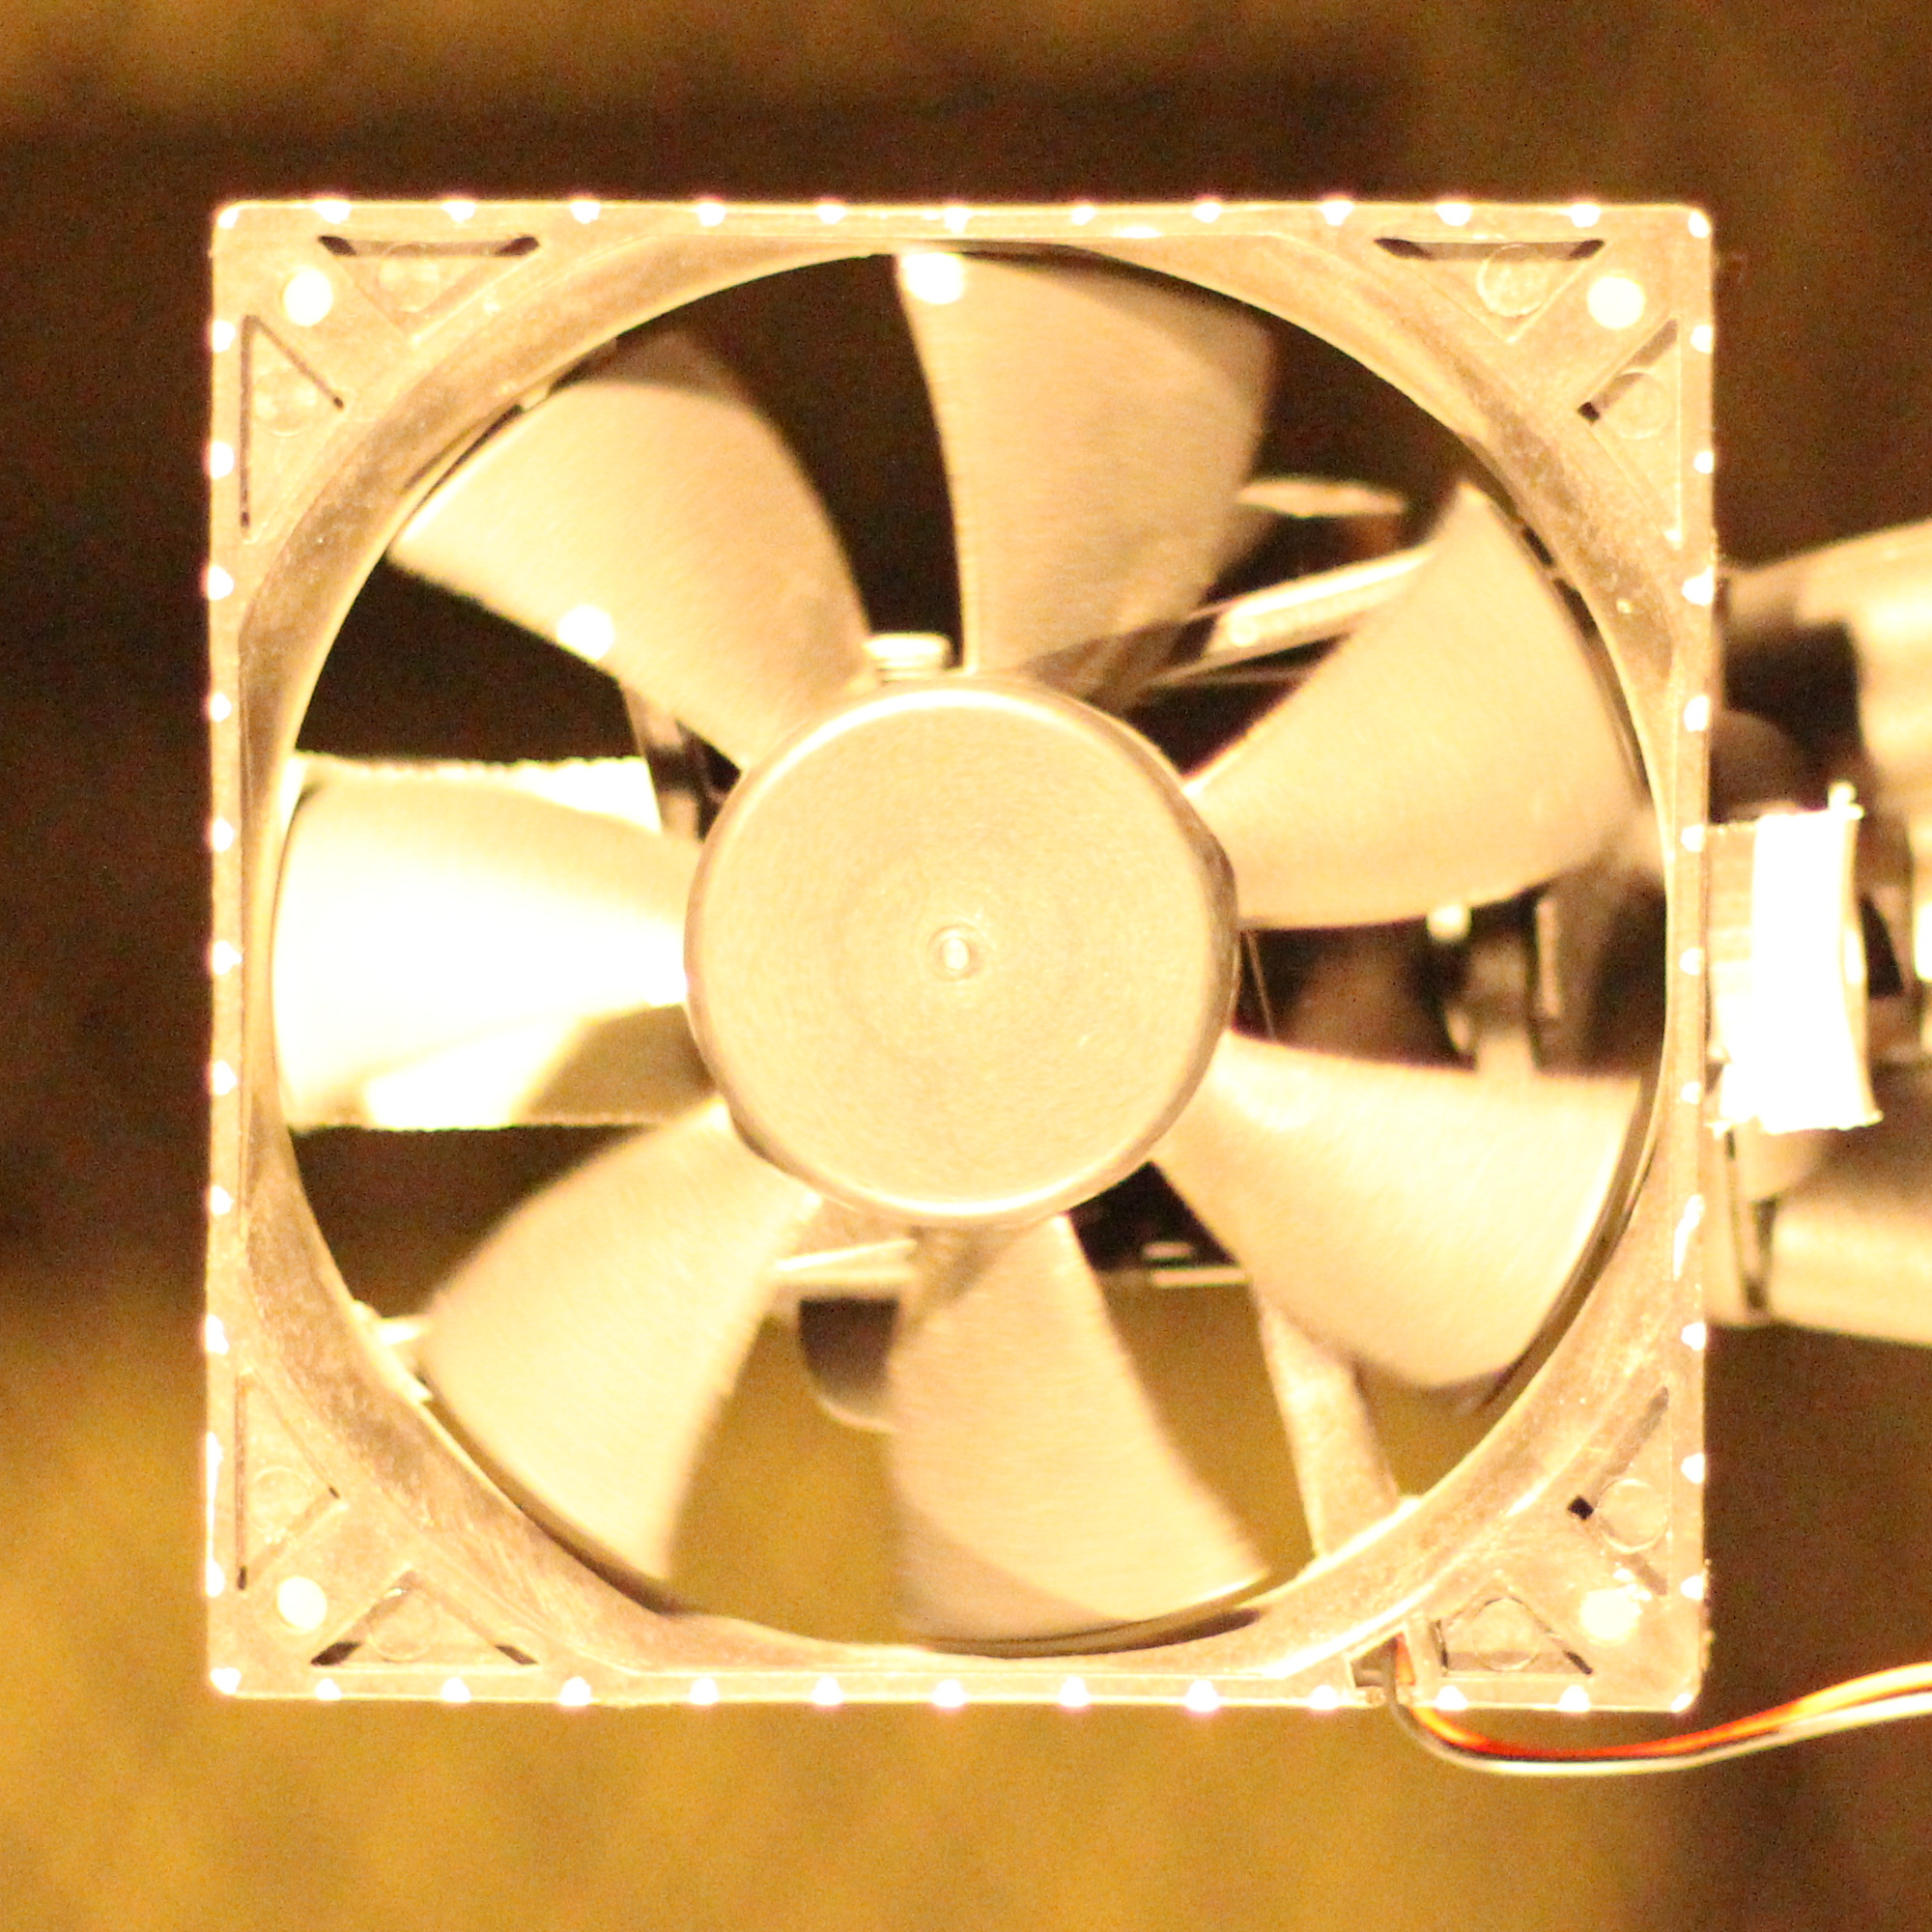
\includegraphics[width=0.45\textwidth]{fan-a}
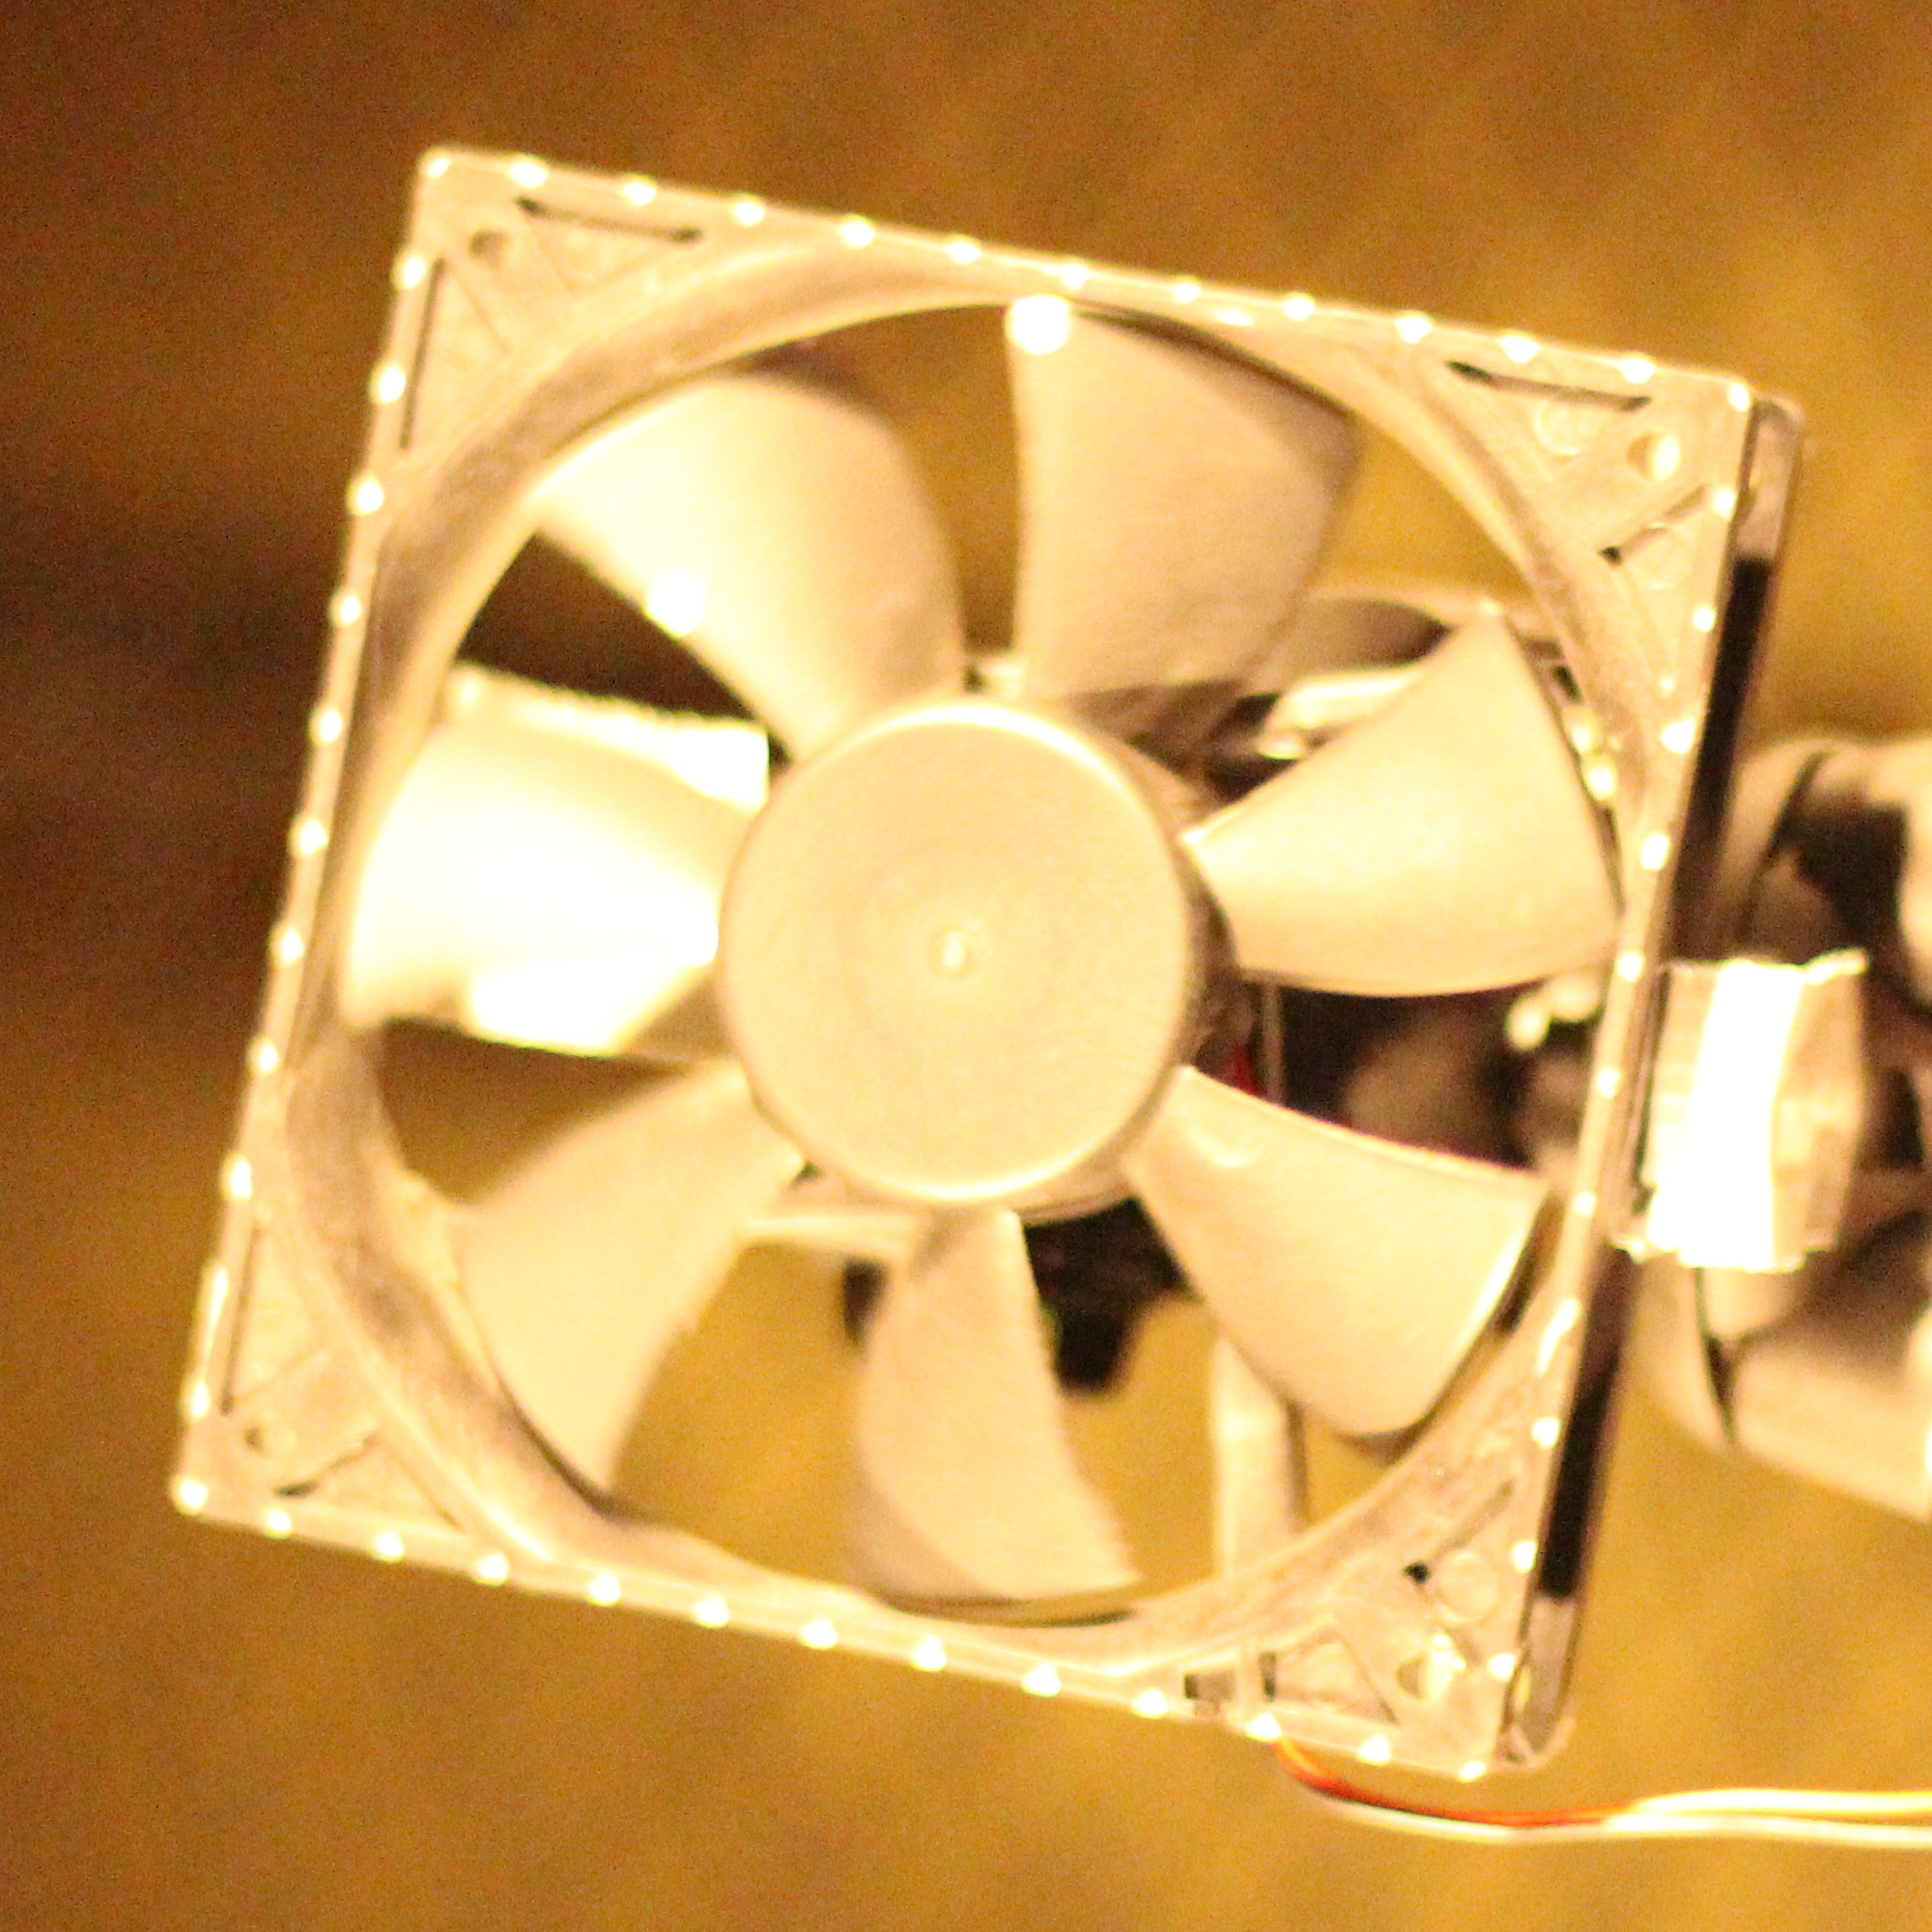
\includegraphics[width=0.45\textwidth]{fan-b}
}{fig:fansynctest}{
	Frames from two cameras in a synchronization test with a PC fan. A marking on the end of a fan blade can be seen in the top.
	The position of the marking does not differ distinctively in the pictures.
}

% "hardly scientific" jonnekin väliin, hehheh?
%Another test was done using a mobile phone microphone.
%A DSLR makes a distinct clanking sound because of its mirror and mechanical shutter.
%Two sound clips were recorded several times: the sound of all cameras triggering at the same time, and for comparison, the sound of a single camera only.
%The waveforms were drawn on top of each other and inspected, and no distinct difference was found.
%For comparison, also intentionally wrongly synchronized sequences were recorded.
%
%\simplegfx{p}{0.8\textwidth}{shutteraudio}{
%	Trimmed audio recordings of all cameras shooting (top), and only a single camera (bottom).
%	The waveforms cannot be clearly distinguished.
%}

\subsubsection{Video capture}

% intro

The EOS 700D does not support an external clock signal for timing the frames in video recording, but relies on an internal clock to sync the frames within a single video file.
It can be safely assumed that the clock speed has little variation, and thus, little drift or jitter occur in the videos.
Recording offset remains an issue:
processing time of each camera from the shutter button to start of first frame varies because of unknown reasons; even though a Canon wireless remote control would be used for starting several cameras at once, the offset was found to be sometimes almost as much as the duration of two frames.

% what was done

Visual and audio-based tests were carried out to find variations in the recording offset.
Three cameras were triggered several times with a Canon RC-6 wireless remote control.
The remote sends a short infrared pulse to a sensor in the front of a camera when a key is pressed.
The cameras were set in video mode and configured to use the remote release.
%The exposure time was set to minimum, 1/4000 s, to maximise the rolling shutter effect.
%In this mode, the sensor rows are exposed one by one in succession.
When all cameras had started recording, a flash unit (Canon Speedlite 420EX) was aimed at the lenses and fired manually several times.

% what happens

A direct light pulse of a flash unit shows up as an over-exposed, completely white video frame, if the whole frame was exposing the image during the light pulse.
Sometimes only part of the frame would be exposed to the flash light as a rolling shutter effect.
Because the CMOS sensor is cleared and read line by line, the time of the flash can be deduced from the first bright line in the image.
The rows are zeroed from light in succession in the same way as a mechanical focal plane shutter moves and exposed until read.
Thus, the flash light's starting time in the video's internal clock is the frame's start time plus the duration that it takes for the rows before the overexposed one to show up:

\begin{align} \begin{split} \label{eq:timingcalib}
t_{Cl} &= t_{Ci} + t_{Cf} \\
&= i_C * F + f_C / R * F \\
&= (i_C + f_C / r * c) * F
\end{split} \end{align}

where $C$ is a camera identifier, $t_{Cl}$ is camera-relative time for the light pulse, $t_{Ci}$ is the starting time for the frame where the light shows up, and $t_{Cf}$ is the time inside the particular frame.
The frame index $i$ marks the number of the frame in the video file, starts from 0, and there is $F$ = $1/\text{fps}$ seconds between the frames.
$f_C$ is the first exposed row, $R = r / c$ is the time for a single row to expose, $r$ is the vertical frame resolution and $c$ is a correction coefficient describing the ratio of exposure time and frame duration ($0.5$ in this case, referring to a characteristic to the camera, as it exposes the first and last rows in half the time between frames).
Offset between two cameras $A$ and $B$ is then $t_{Al} - t_{Bl}$.
The timings are depicted in Figure \ref{fig:flashtimeline} as a timeline with matching symbols.

For perfectly synchronized videos, the frames would be identical, and time difference calculated with eq. \ref{eq:timingcalib} for each frame would be zero as $i_C$ and $f_C$ would be constants for all $C$.

\simplegfx{h}{1.0\textwidth}{flashtimeline}
{Illustration on timing calibration of two cameras using a flash light.
The darkened areas represent the exposure times and the red band represents the light pulse.
In this example, $c = 0.5$.
}

\simplefig{p}{%
\setlength\fboxsep{0pt}
\setlength\fboxrule{1pt}
\fbox{
\includegraphics[width=0.3\textwidth]{flashtiming-a}}
\fbox{
\includegraphics[width=0.3\textwidth]{flashtiming-b}}
\fbox{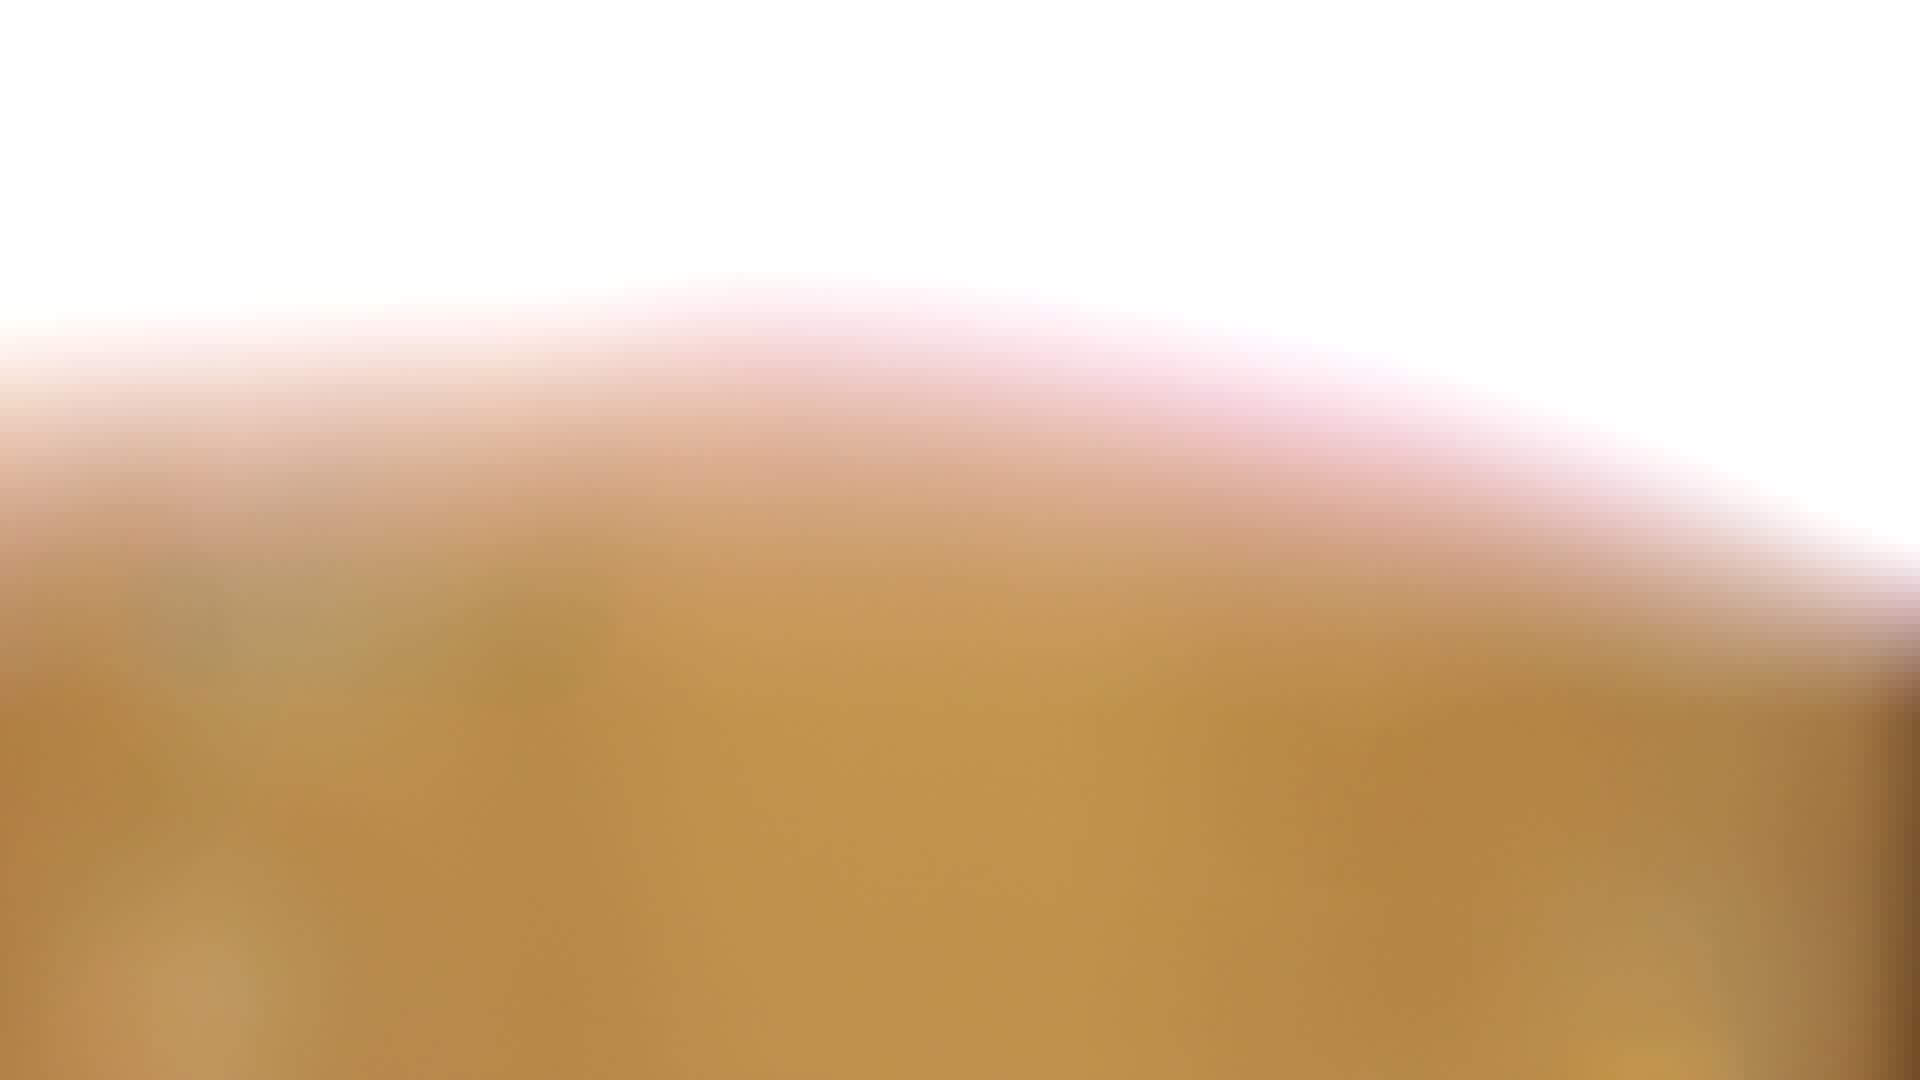
\includegraphics[width=0.3\textwidth]{flashtiming-c}}
}{fig:flashtiming}{
	Video frames of three cameras started with the same remote controller, with the same frame index.
	The time for the flash unit to reach maximum brightness is almost instant.
	The start of the light pulse can be seen in the two last frames.
	In the first, the flash has been fired before the frame exposure started, and the frame shows the flash shutting down;
	the frame before it is without any overexposed light.
	It is impossible to deduce the exact time in this case.
}

\simplegfx{p}{0.8\textwidth}{flashaudio}{
	Trimmed audio recordings near the same moment as in Figure \ref{fig:flashtiming}, extracted from the video files, in top-bottom order.
	First rows of the frames have been exposed at approx. $t = 0.03 \text{ s}$.
	The flash outputs a distinct ``pop'' sound, comparable to the start of the bright part in Figure \ref{fig:flashtiming}.
}


The method for measuring the synchronization error at a sub-frame precision can be used to calibrate the differences, which is useful in artificial sync with optical flow or other methods, where frame timing is used.
A similar method using the recorded audio (as in Figure \ref{fig:flashaudio}) is more used in video photography \cite{pluraleyes,premierepromerge}, where similarities in the sound of the audio tracks recorded by the different cameras would be used for shifting the videos so that their clocks is in sync.
For a small number of cameras, the audio tracks are simple to align manually in an audio editing software, or automatically with cross-correlation to find the time lag.

Another method for triggering multiple video recordings is to use a Magic Lantern based wired remote trigger by pressing the half-shutter, or focus button when a record key has been configured in ML to start recording.
This method did not show any improvements in overcoming the offset, as opposed to the wireless remote.
% it may be even worse, as the additional code in ML induces more lag.

A typical measurement result is shown in Figure \ref{fig:flashtiming}.
Audio recorded by the cameras' internal microphones at the same event is shown in Figure \ref{fig:flashaudio}, and the order of flash pulses in the three frames can be verified from the order of the sound emitted by the flash.
Both methods show that the leftmost shown camera has started recording first, and subsequent time lags compared to it are approximately 21 and 31 milliseconds.
A relatively long exposure time was used.

From the results tested, it was deduced that the Canon EOS 700D implements exposure time in a similar way as a physical focal plane shutter with two artificial curtains, where the first curtain clears each particular sensor row, and the second curtain reads out the accumulated charge.
For a shorter exposure time, a shorter white overexposed line occurs in the video frames, but the scanning speed remains the same.
For this reason, decreasing the exposure time only helps in motion blur, but not in rolling shutter artifacts.

\subsection{Sample subjects} \label{sec:samplesubjects}

%The mask, human heads, legos, books

Test subjects were scanned using the system for validation and analysis.
Different datasets were used on two popular reconstruction software pipelines.
Proposals for a typical scanning setup and minimum quality of instant results are shown in this section.
The results answer questions on what kinds of surfaces can be reconstructed well; different types of materials are given for the datasets.
It was expected that areas with low texture or high reflectivity would pose most problems.
No particular tuning of any algoritmic configuration parameters were tested, which suggests that higher quality than that of presented here can be achieved with more careful work.
No makeup, light polarizers or any such improvements were tested; the subjects were photographed as-is in normal lighting.

The system is flexible to extend for complete body scanning with limited accuracy; tests for such subjects were left out due to lack of time and space in the hall where the system was used.
For a complete body, the methods are identical but as the distance to the subject is greater, less detailed geometry is expected to result.

\subsubsection{Photography setup}

The nine cameras were set up in a dark hall as a $3 \times 3$ grid and two flash units were attached to two cameras, directed up and down to a white styrofoam board and a fabric diffuser to soften the light, shown in Figure \ref{fig:setupcams} and Figure \ref{fig:frontview}.
The flash units were a Canon Speedlite 430EX and a Yongnuo YN565EX II, set to normal front curtain sync.
The top-facing Canon flash has only automatic mode, which was sufficient; the Yongnuo was set to manual full power, facing downwards to a piece of fabric.
The Canon EOS 700Ds have internal pop-up flash lights; they were not used, as they were found to trigger inconsistently, and they are relatively too bright and small so that dark shadows and highlights would pose a problem.

A black background matte was used to isolate out unnecessary items in the background;
the textureless out-of-focus fabric has no particular features that would be detected, and its color is not particularly important, although chroma-keying with a green cloth is commonly used to isolate the subject already in the source images.
White styrofoam boards were left to the sides of the rig to help with lighting.
The general setup is shown in Figure \ref{fig:totalsetuptwo}, and a closer depiction of the poses of the cameras and the flash unit bounced from downwards are shown in Figure \ref{fig:frontview}.

\simplefig{p}{%
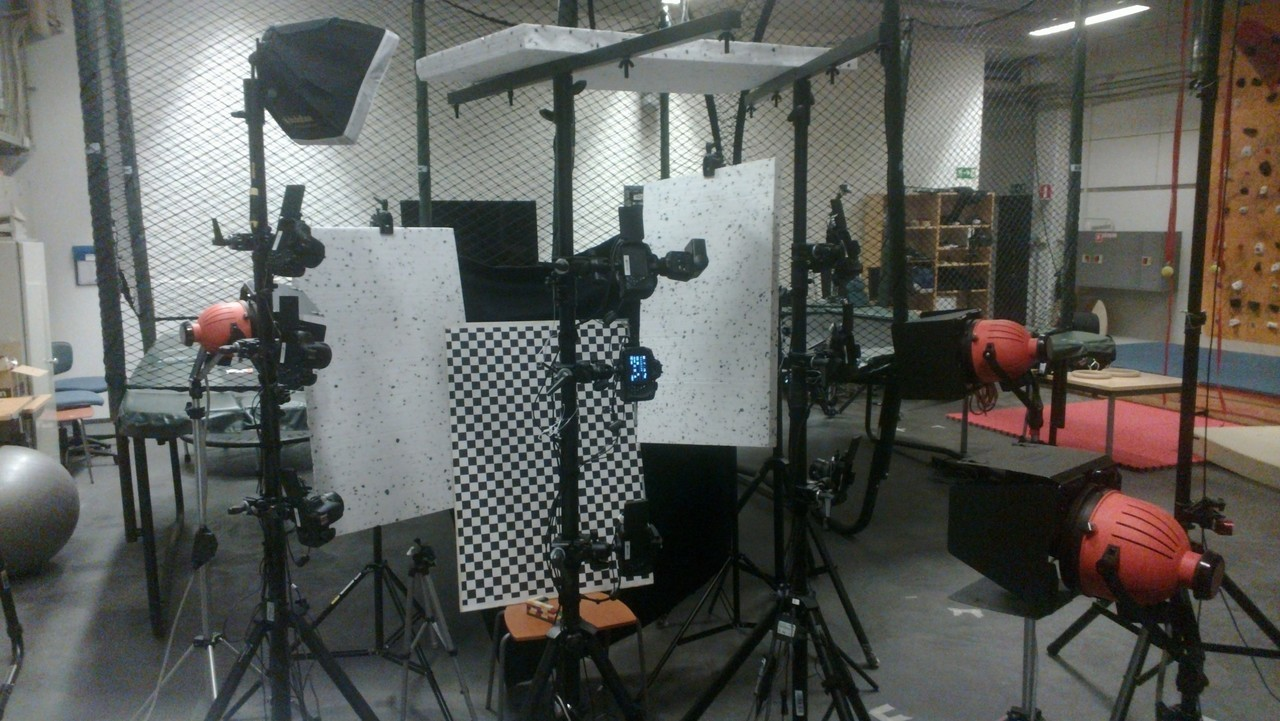
\includegraphics[width=\textwidth]{totalsetup}
}{fig:totalsetuptwo}{
	Complete setup with cameras mounted on the stands, surrounded by 800 watt spot lights (red) for video recording tests.
}

\simplefig{p}{%
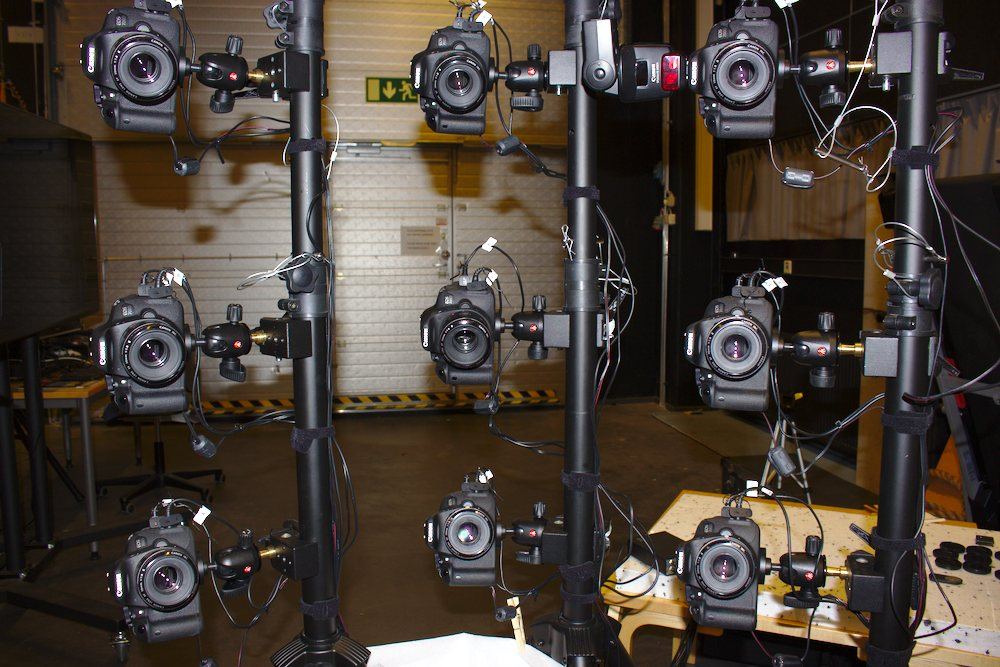
\includegraphics[width=0.45\textwidth]{setupcams}
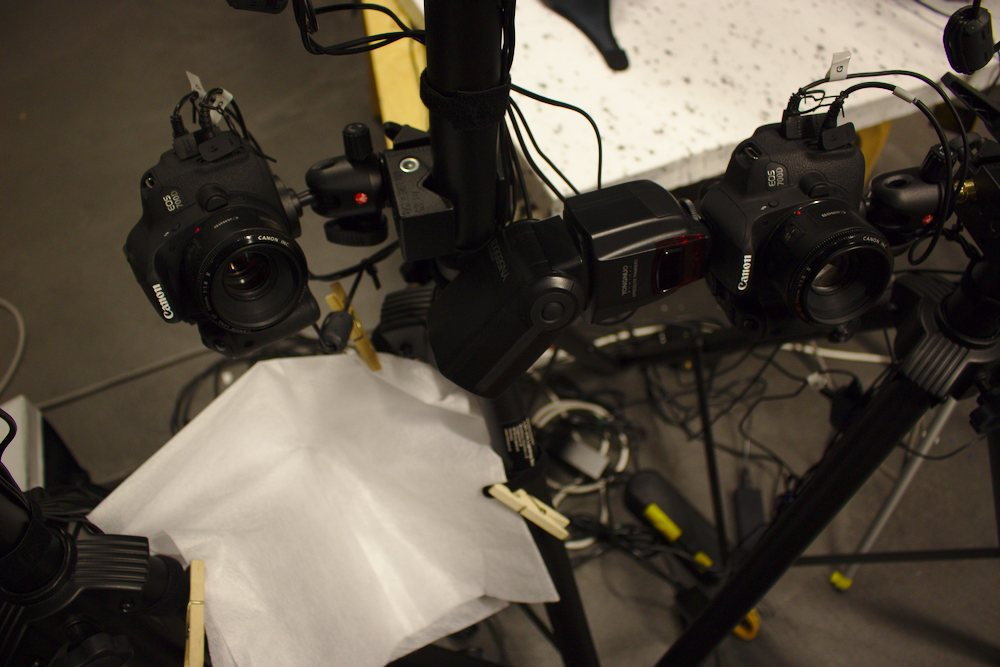
\includegraphics[width=0.45\textwidth]{flashbounce}
}{fig:frontview}{
	Left: Poses of the cameras from the subject's viewpoint.
	Right: Flash gun bounced from a white cloth is used to evenly illuminate the bottom side of the subject.
}

%\simplegfx{p}{0.5\textwidth}{setupcams}{
%	Poses of the cameras from the subject's viewpoint.
%}
%
%\simplegfx{p}{0.5\textwidth}{flashbounce}{
%	Flash gun bounced from a white cloth is used to evenly illuminate the bottom side of the subject.
%}
%


The Bundler SfM system recommends to take photos at least every $\alpha = 15$ degrees around a subject \cite{bundlerfaq}.
Similar rough guidelines are usually suggested, such as a camera baseline of 10-20 \% of the distance to the subject.
% visualsize photomodel3d recommends 12 degrees http://www.visualsize.com/FAQ/3Dmodel.php
With a distance $d$ of one metre from lens to the subject, the Bundler guideline yields a baseline $b$ of approximately 26 cm by Equation \ref{eq:baselinedegrees}:

\begin{align} \begin{split} \label{eq:baselinedegrees}
	\sin \alpha/2 &= \frac{b/2}{d}\\
	b &= 2 d \sin \alpha/2
\end{split} \end{align}

The key camera parameters used for photographing most samples are listed in Table \ref{tab:sampleshotparams}.
In a dark environment with flash lights, the exposure time is not particularly important for a static subject; the short flash pulse dominates all light in the scene.
The baseline was chosen by the guidelines proposed and by the difficulty in using the cameras in close proximity to each other.
Initially, a slightly longer baseline of approximately 50 cm was used; it was furthermore reduced to 30.

\begin{table}[h]
	\centering
	\begin{tabular}{l l}
		Camera baseline & 30 +/- 5 cm\\
		Aperture size & f/14\\
		Exposure time & 1/20\\
		ISO sensitivity & 200\\
		Subject distance & 90 +/- 10 cm\\
		Lighting & Two flash heads bounced indirectly\\
		Focusing & Automatic\\
	\end{tabular}
	\caption{
		Key parameters in the sample photographs.
		Baseline refers to the distance to the nearest camera, horizontally and vertically.
	}
	\label{tab:sampleshotparams}
\end{table}

\paragraph{Reconstruction software}
Two different popular pipelines were used on the photography results.
Agisoft PhotoScan is a self-contained pipeline, and VisualSFM does only part of the SFM reconstruction, leaving much work to external programs that it runs automatically, providing flexibility in selecting the different algorithms.
The two programs were chosen among others based on popularity and availability.

PhotoScan \cite{photoscan} is a popular commercial program for scanning subjects from several pictures for generation of 3D models and measuring spatial data.
Agisoft advertises PhotoScan ``to be used in GIS applications, cultural heritage documentation, and visual effects production as well as for indirect measurements of objects of various scales''. \cite{photoscan}
%The programs are targeted for the end user and include tools for editing the resulting data, and need no external tools for outputting complete meshes.
A free demo version was used, which does not include exporting the generated meshes; screenshots were taken in the user interface for illustration of results.

PhotoScan uses a typical multi-view reconstruction pipeline, optimized for speed and taking into account practical issues such as light variations.
The steps consist of photo matching, camera parameter estimation, dense reconstruction, mesh generation and texture mapping.
No detailed description is available on the implemented algorithms. \cite{photoscanalgorithms}

VisualSFM \cite{visualsfm} performs the same structure from motion estimation and dense point cloud generation by combining several research projects into a single graphical user interface.
The work pipeline in VisualSFM is composed in parts that are done mostly by external programs; feature extraction and matching is done first using SiftGPU \cite{chengchang2007siftcpu}, followed by SfM using PBA \cite{wu2011multicore}, and finally dense reconstruction is performed by PMVS/CMVS \cite{furukawa2010accurate,furukawa2012patch} (CMVS always resulted in only a single cluster due to the small number of views).
Final Poisson surface reconstruction is done by opening the resulting dense point cloud in Meshlab and using its reconstruction plugin. \cite{meshlab}

PMVS works by expanding a set of initially found patches iteratively in the reconstruction, resulting in a dense point cloud with oriented and colored points.
The point cloud is filtered by certain visibility constraints, and the resulting points have few outliers. \cite{furukawa2012patch}.

PMVS divides the source images iteratively to smaller sets, and begins at a halved size by default with one fourth of the pixel count of the original.
Forcing the original size was found to provide roughly twice the amount of points with four times longer processing time, but with no increased accuracy.
The documentation of this parameter also suggests that a halved size is used, because a large part of colors are interpolated in the original image because of the color filter array in the image sensor (Section \ref{sec:sensors}).

No software installation instructions are provided in this thesis; refer to documentation of the presented programs for installation and usage.
All photographs were captured using the developed software presented in the previous Section \ref{sec:implementation}.

\subsubsection{Static subjects}

With the 18 million pixel count of the cameras, a human face is scanned with pore-level detail, and no markers are necessary.
Markerless capture has been suggested to be important for human subjects, as both the geometry and the texture can be scanned simultaneously, and variations of the texture over time are also seen when capturing video. \cite{bradley2010high}

\paragraph{PhotoScan results}
Using the source data shown partly in \ref{fig:sample-arto-photoscan-source}, a point cloud and a textured mesh were generated in PhotoScan, using a quality setting of ``High''.
The workflow in PhotoScan is similar to that of VisualSFM and other tools based on separate programs:
initially, the scene structure is computed, resulting in a sparse point set of the subject and camera parameters.
A dense point set computation is followed, and finally a textured triangle mesh is computed based on the dense points and source images.
Spatially uniform quality in the point cloud suggests that all PhotoScan's algorithm uses all cameras in a combined way, instead of e.g.\ computing disparity maps in pairs and naively combining the maps.

Figure \ref{fig:sample-arto-photoscan} depicts the results from a dense point cloud and a textured mesh based on the point cloud.
A typical face scan with surrounding geometry removed results in a high-density point cloud of 2-3 million points, which the software reduces into a textured mesh with exactly five times less triangles than the original points.
The meshing process was found to consume temporarily 4-5 GB of RAM on a typical human subject.

PhotoScan was found to be relatively robust to baseline length, reconstructing the scene geometry well with a baseline almost twice as much as the 15 degree rule suggested in Bundler with no apparent increase in accuracy or matching performance when the baseline is halved.
The tested reconstructions in PhotoScan have significant noise on all point sets and surfaces for unknown reasons, though.
By the console output of the mesh generation process, the meshing algorithm is probably based on Poisson surface reconstruction or similar octree based algorithm.

The resulting point set is dense enough to include medium wrinkles in the reconstructed mesh geometry, but with a well noticeable level of noise, larger than the smallest pore-level details seen in the photographs.
Medium-scale wrinkle detail tests can be seen in Figure \ref{fig:sample-arto-forehead}; the point cloud and the mesh have enough detail to encode forehead wrinkles in the geometry, in addition to the texture color.

In Figure \ref{fig:sample-arto-photoscan-textures}, two of the texture mapping modes provided by PhotoScan are depicted.
A ``generic'' mapping mode with no distortion in the pictures produces piecewise texture islands with original photo content.
A ``spherical'' mode where the subject is assumed to be a sphere and the texture is made continuous but the original photos are warped shows as more intuitive and easier to modify manually if necessary.

%As seen in Figure \ref{fig:sample-arto-forehead}, the triangle mesh is more detailed than what would typically be used by an end-user; the small skin wrinkles that show as color variations would be rendered as variation in the texture color.

\simplefig{h}{%
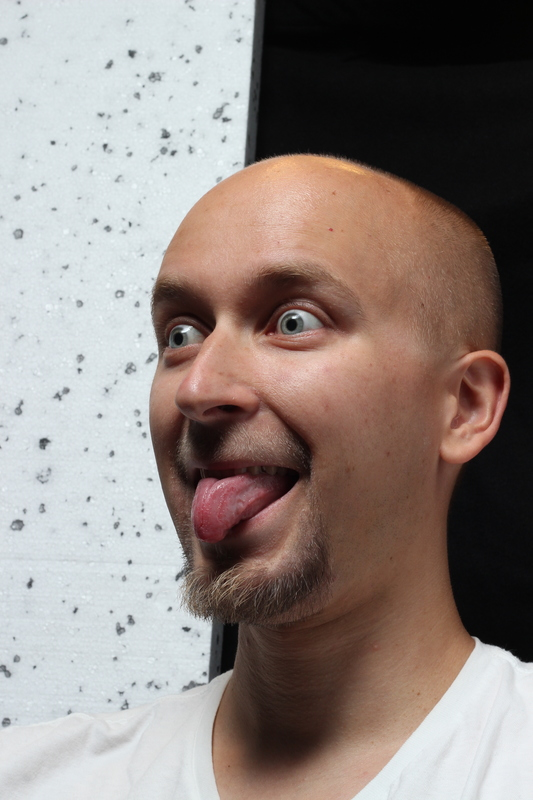
\includegraphics[width=0.3\textwidth]{arto-1}
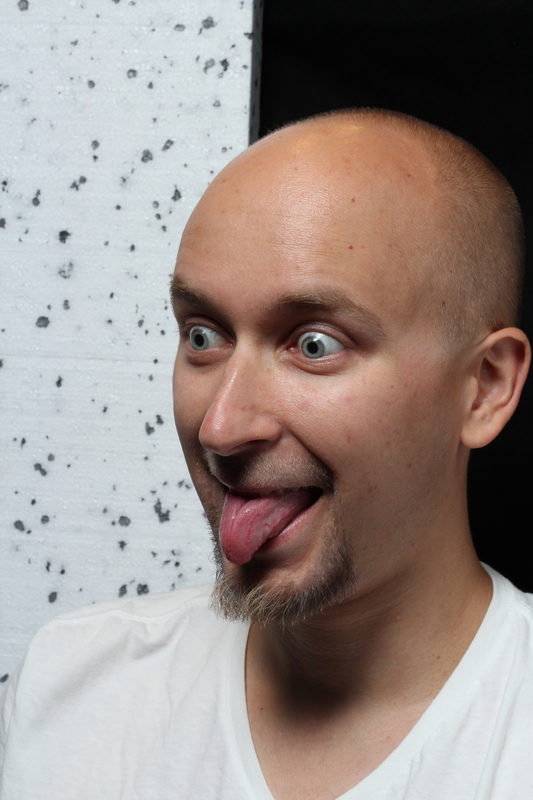
\includegraphics[width=0.3\textwidth]{arto-2}
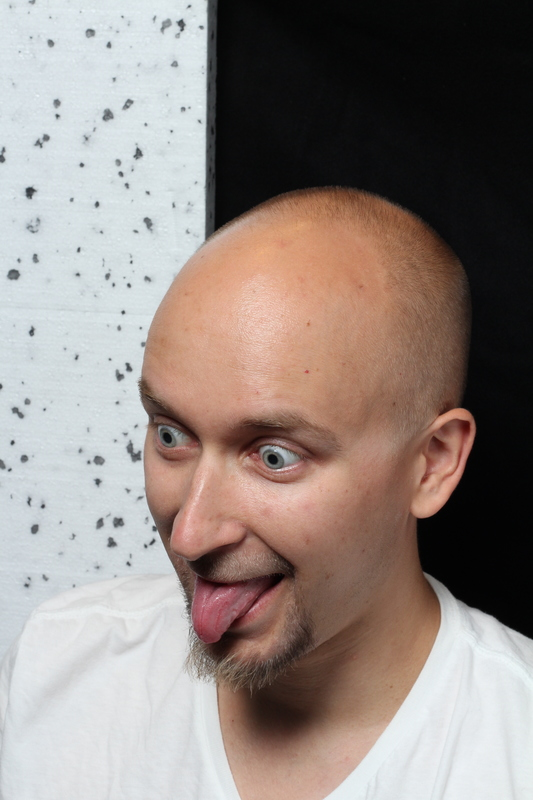
\includegraphics[width=0.3\textwidth]{arto-3}
}{fig:sample-arto-photoscan-source}{
	Three of the nine source pictures for a typical scan;
	for a more optimized scan, the subject should be closer to the rig to use the full frame.
	Note the shadows under the chin, the nose, and near the eyes; only the top flash was used for this dataset for demonstration.
}

\simplefig{h}{%
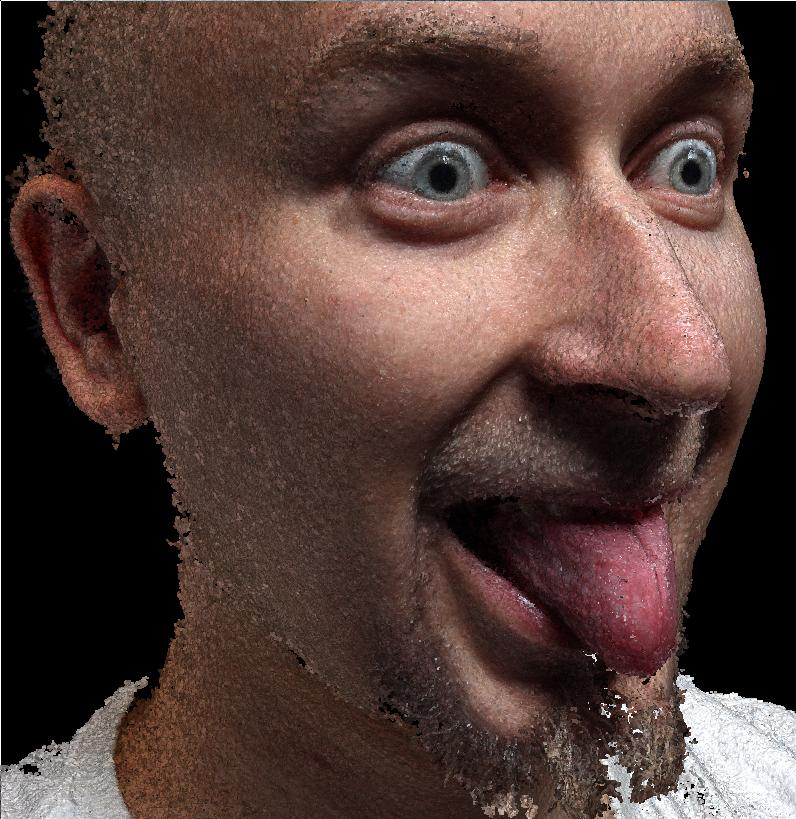
\includegraphics[width=0.5\textwidth]{photoscan-arto-dense}%
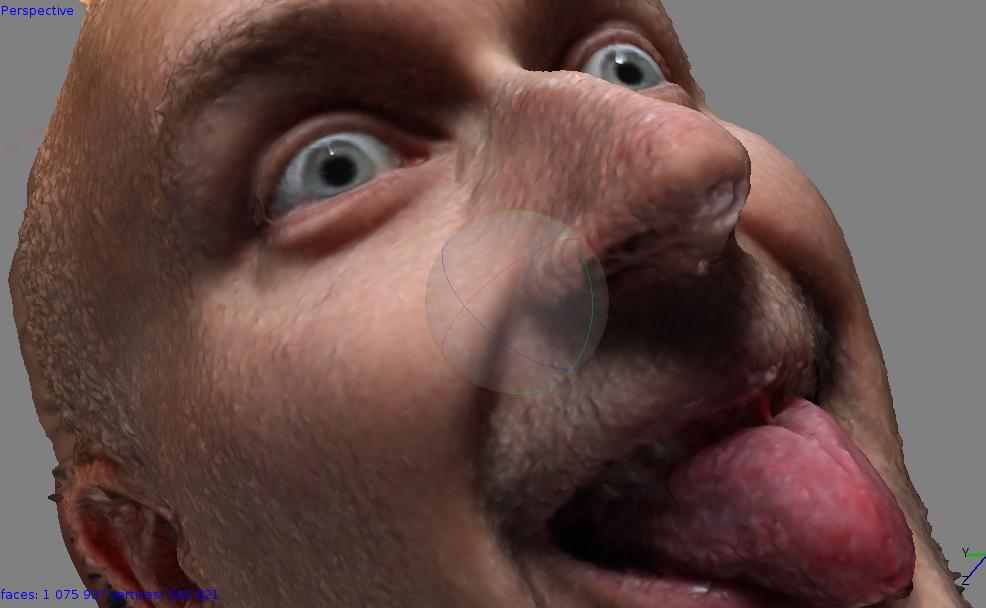
\includegraphics[width=0.5\textwidth]{photoscan-arto-textured}
}{fig:sample-arto-photoscan}{
	A dense point set (left) and a textured mesh in PhotoScan, matching the pictures in Figure \ref{fig:sample-arto-photoscan-source}.
	The underlying triangle mesh contains as much noise as the point set, which is hidden by the noiseless texture.
}

\simplefig{h}{%
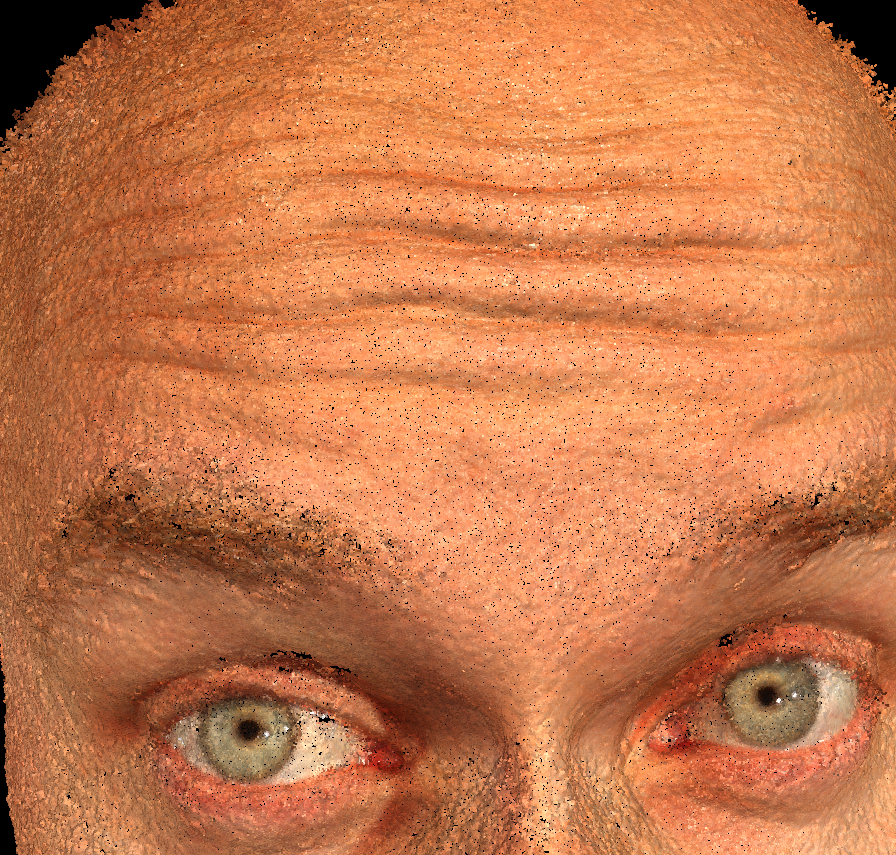
\includegraphics[width=0.5\textwidth]{arto-forehead-dense}%
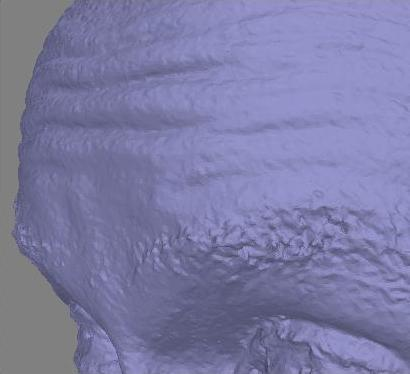
\includegraphics[width=0.5\textwidth]{arto-forehead-solid}\\%
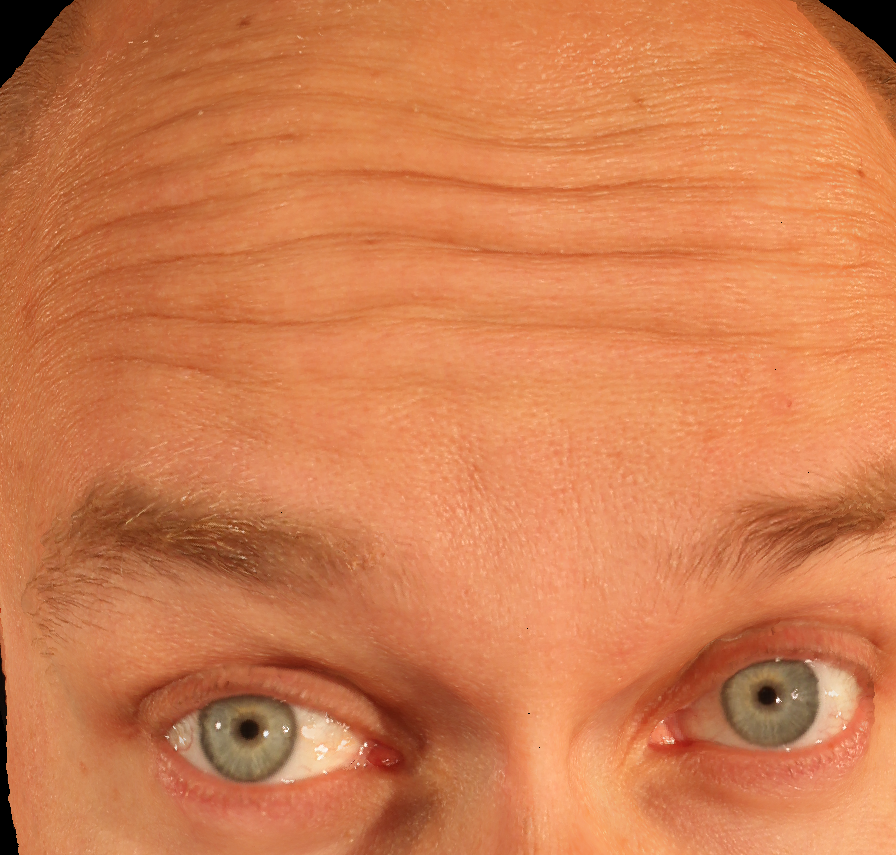
\includegraphics[width=0.5\textwidth]{arto-forehead-tex}%
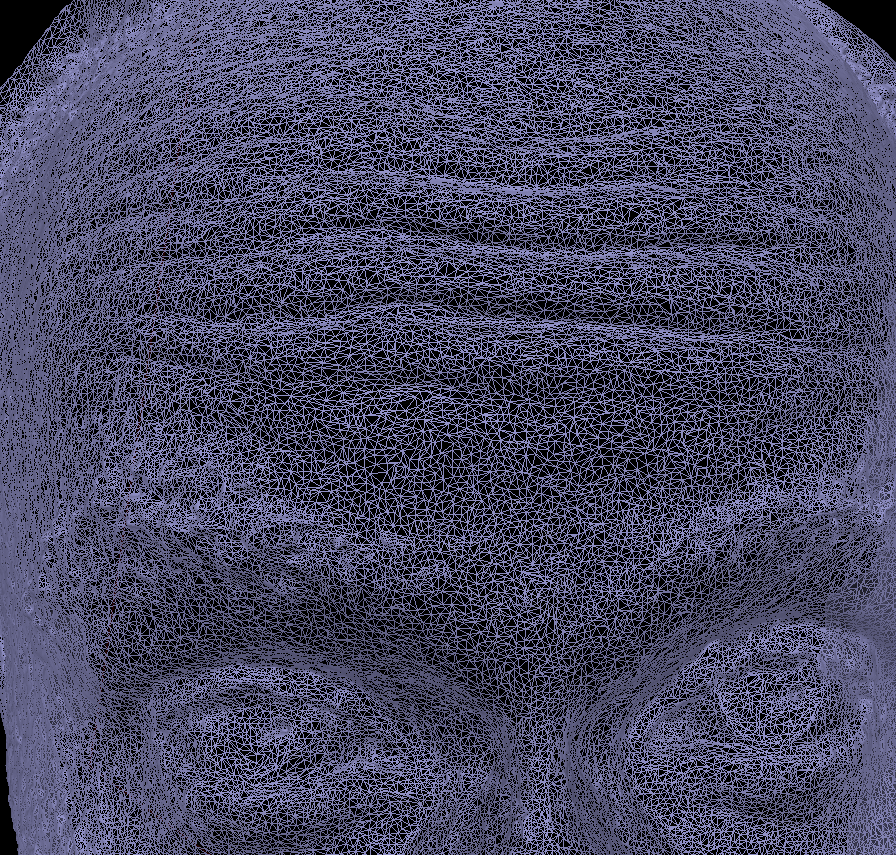
\includegraphics[width=0.5\textwidth]{arto-forehead-wireframe}\\%
}{fig:sample-arto-forehead}{
	Forehead wrinkles in PhotoScan: dense point cloud, solid mesh, textured mesh and a wireframe mesh.
	The point cloud and wireframe pictures show the reconstructed detail level well.
	The darkened color due to shadowing in the wrinkles is directly encoded in the color texture.
}
\simplefig{h}{%
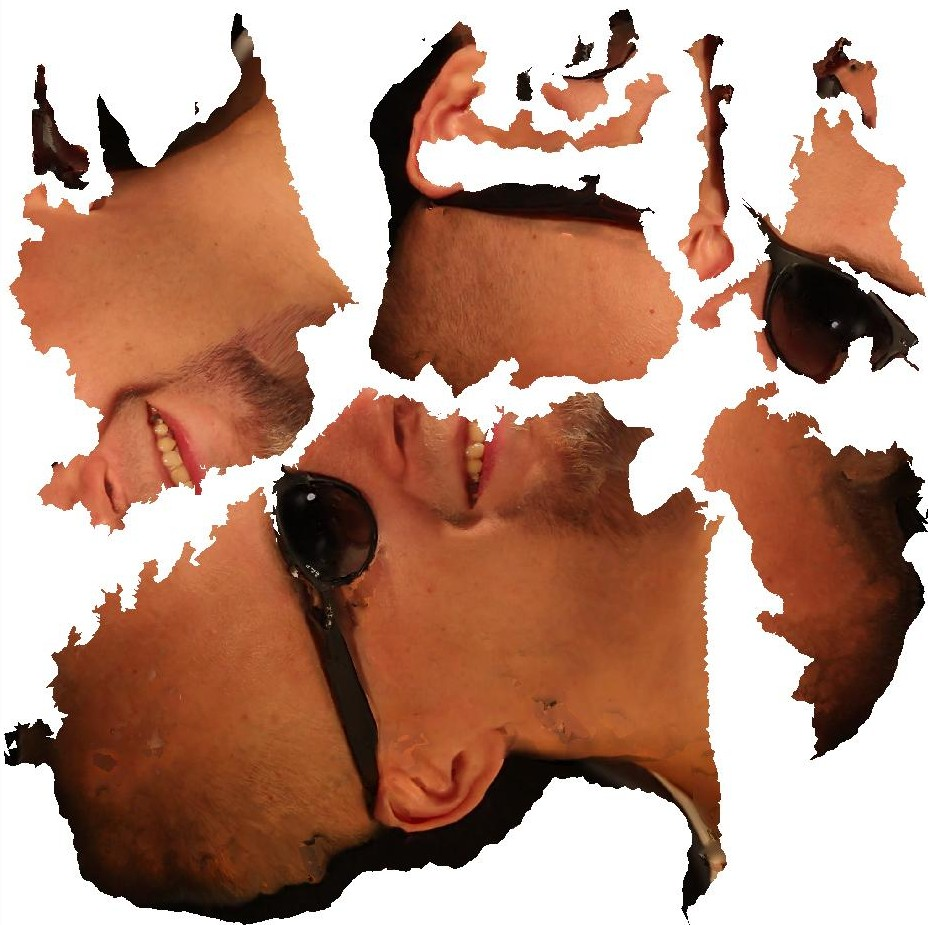
\includegraphics[width=0.45\textwidth]{artoglassuvgeneric}%
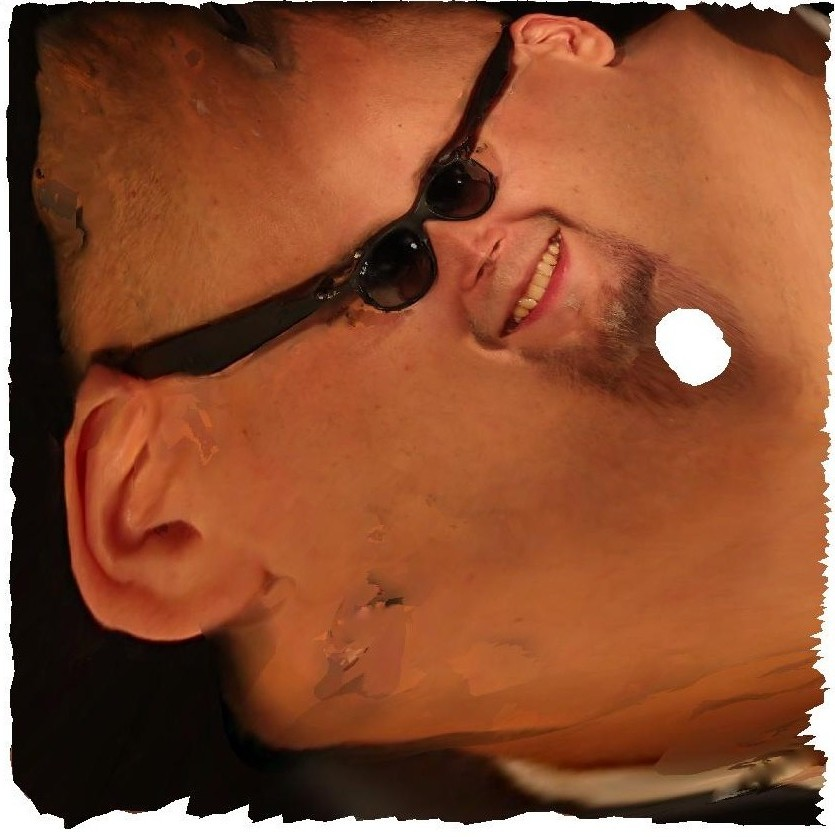
\includegraphics[width=0.45\textwidth]{artoglassuvspherical}
}{fig:sample-arto-photoscan-textures}{
	The ``generic'' (left) and ``spherical'' (right) texture mapping modes in PhotoScan.
	The missing spot under the chin is a result of poorly set up cameras that should have been set lower for more visibility.
}

\simplefig{h}{%
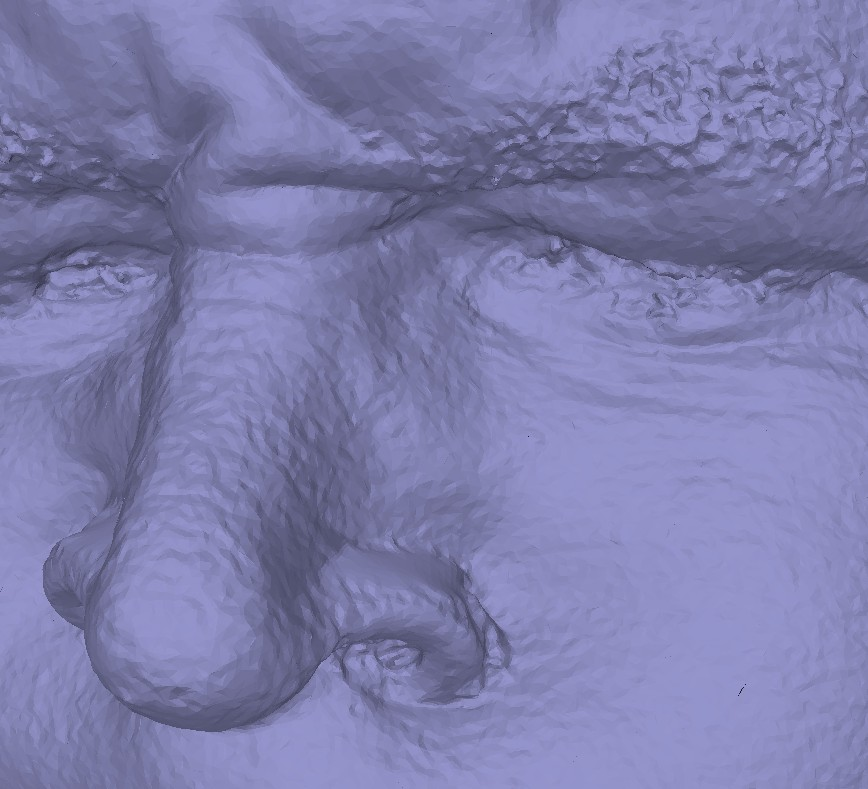
\includegraphics[width=0.45\textwidth]{photoscannose}
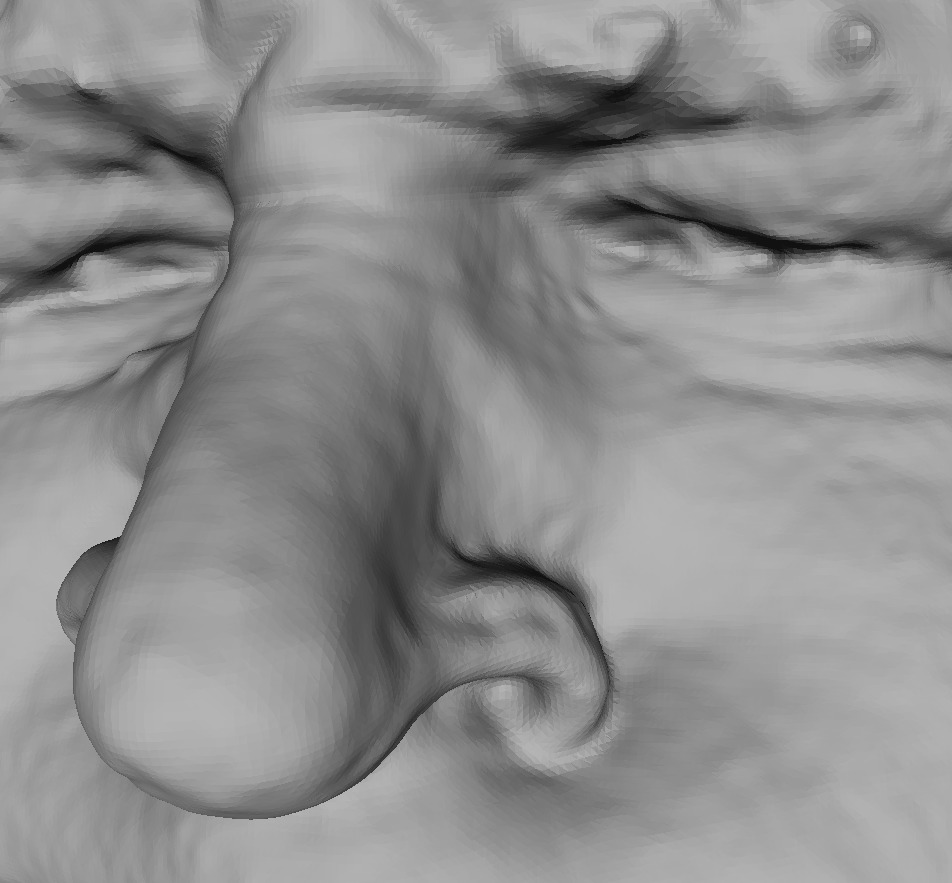
\includegraphics[width=0.45\textwidth]{meshlabnose}
}{fig:soodaheadclosecompare}{
	Surface smoothness comparison.
	The mesh from Meshlab (right) is visually more smooth than the mesh from PhotoScan, while the polygon count is approximately the same.
	Although not as visible, the same could be seen in the point clouds (not shown).
}

%\simplefig{h}{%
%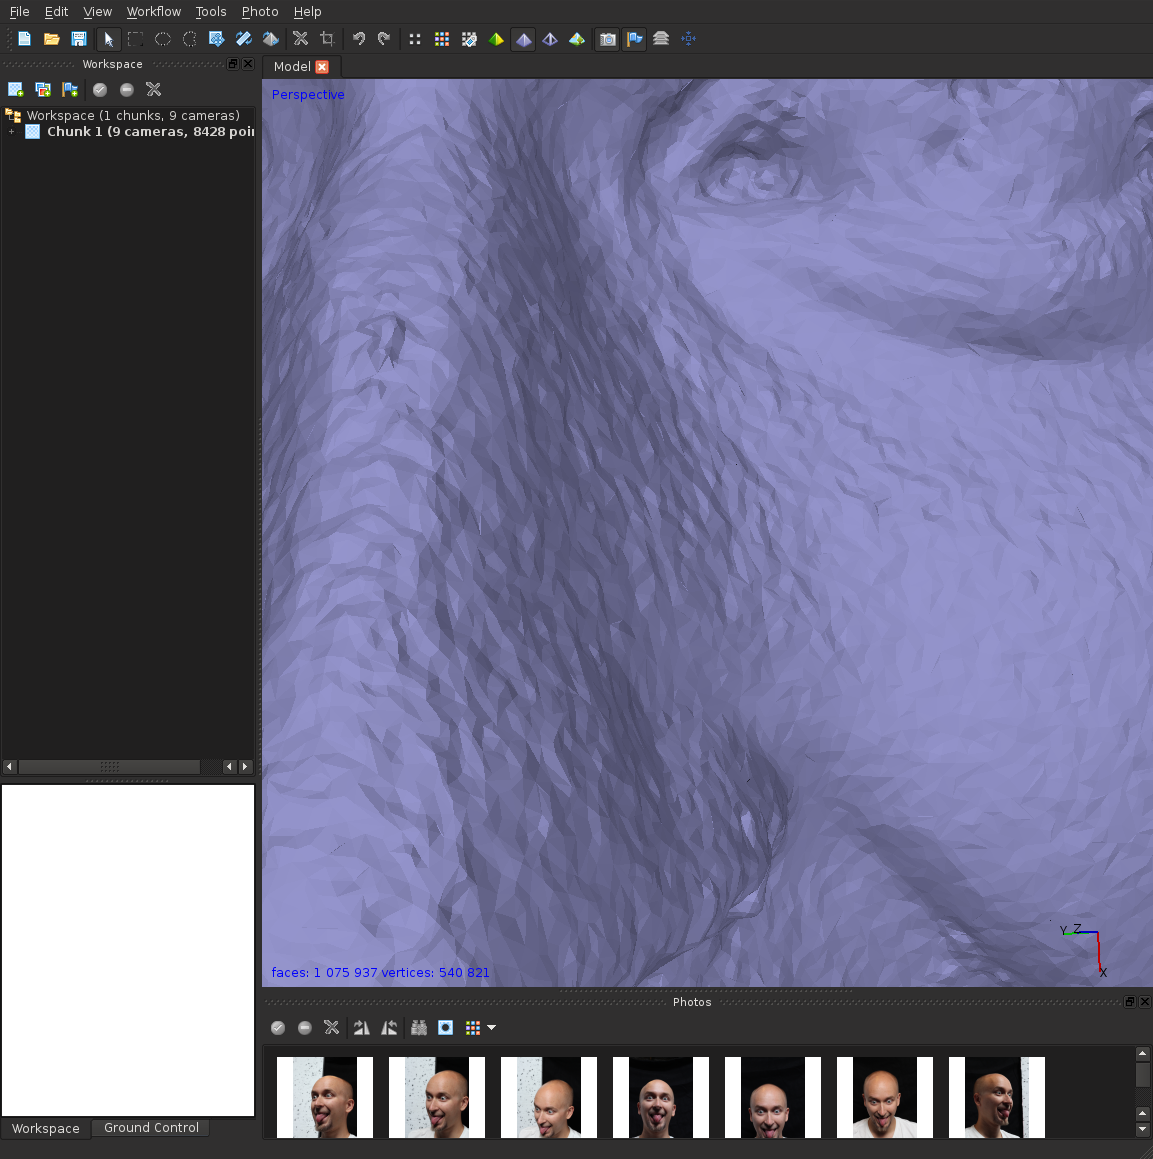
\includegraphics[width=0.38\textwidth]{arto-dense-close-solid}
%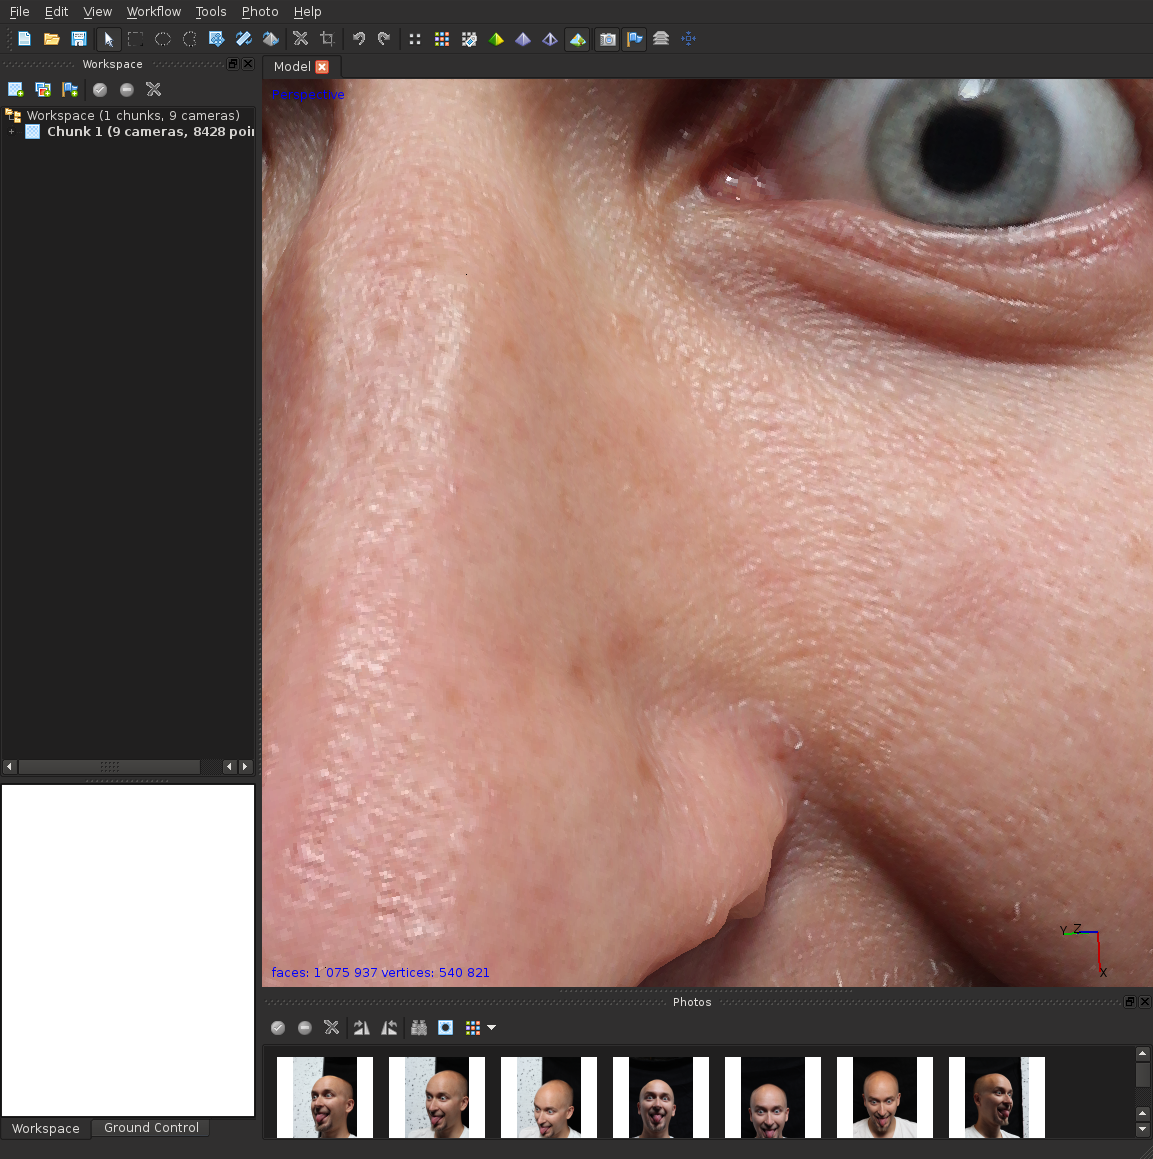
\includegraphics[width=0.38\textwidth]{arto-dense-close-tex}\\
%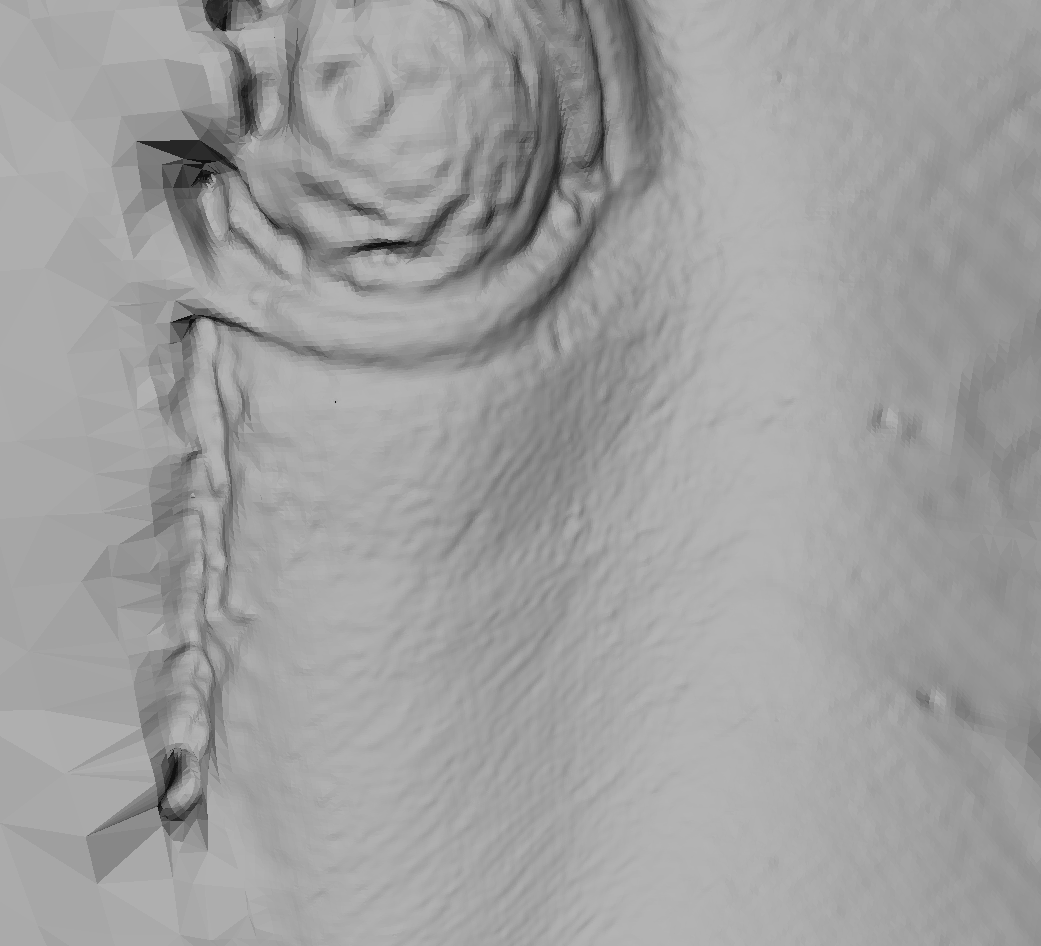
\includegraphics[width=0.38\textwidth]{horseclose-solid}
%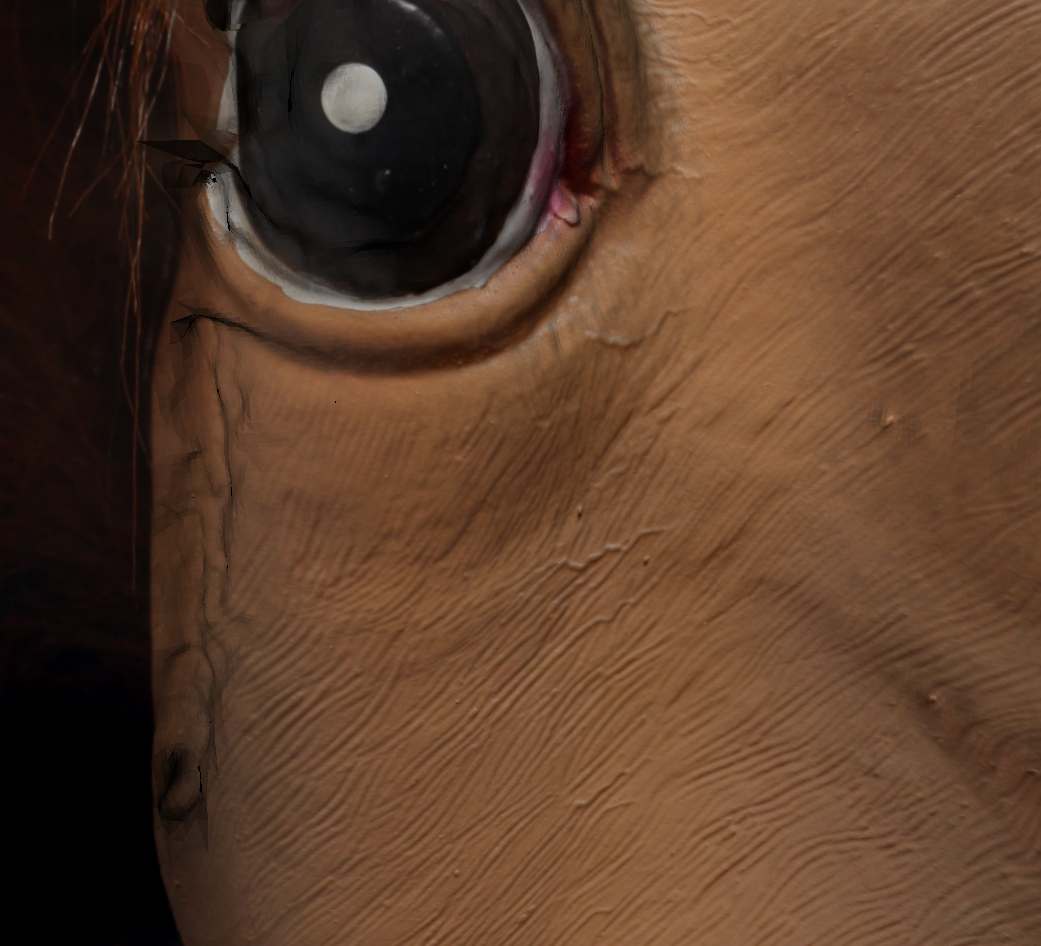
\includegraphics[width=0.38\textwidth]{horseclose-tex}
%}{fig:soodaheadclosecompare}{
%	Surface smoothness comparison.
%	Top: PhotoScan.
%	Bottom: Meshlab.
%}
\paragraph{VisualSFM and Meshlab results}
This alternative was found to be slightly faster than PhotoScan, while the resulting geometry also contains fewer, but more accurate points.
Same datasets were tested as with PhotoScan with similar results.
VisualSFM's feature matching seems not as robust as with PhotoScan, sometimes resulting in separate models because of a too long baseline and displaying very few feature matches between pictures.
The VisualSFM manual suggests to decrease the camera baseline in this case or to take more pictures.
With the shorter baseline of approximately 30 cm, the SfM process was consistently successful.
This suggests that the SIFT feature descriptor may not be the best for this purpose, if it does not cope well with different viewpoints.

The results of a face scan are depicted in Figure \ref{fig:sample-sooda-meshlab}; the surface has visibly less noise than that of PhotoScan's, but without a ground truth geometry, precise analysis is not possible.

Figure \ref{fig:soodaheadclosecompare} shows a cropped region of one of the source photographs.
Note that the skin pores and wrinkles are visually well noticeable in the photograph, but the triangular model is missing smallest of them.
High-level detail could be encoded in the color texture as it shows in the photographs, but since the detail is geometric, computer renderings using detailed light models in differently lit environments need geometric information of the surface roughness, not only a color texture.
The texture type built in Meshlab is depicted in Figure \ref{fig:meshlabtex}.

Beeler et al. propose a mesoscopic augmentation from the captured color images to increase the geometric detail level, and point out that they are not reconstructed to the surface only because of a too small camera resolution. \cite{beeler2010high}
As high level of geometry as produced initially by the surface generation process may not be necessary if the color images are analyzed for producing textures describing the surface roughness level with texture mapping.

\simplefig{h}{%
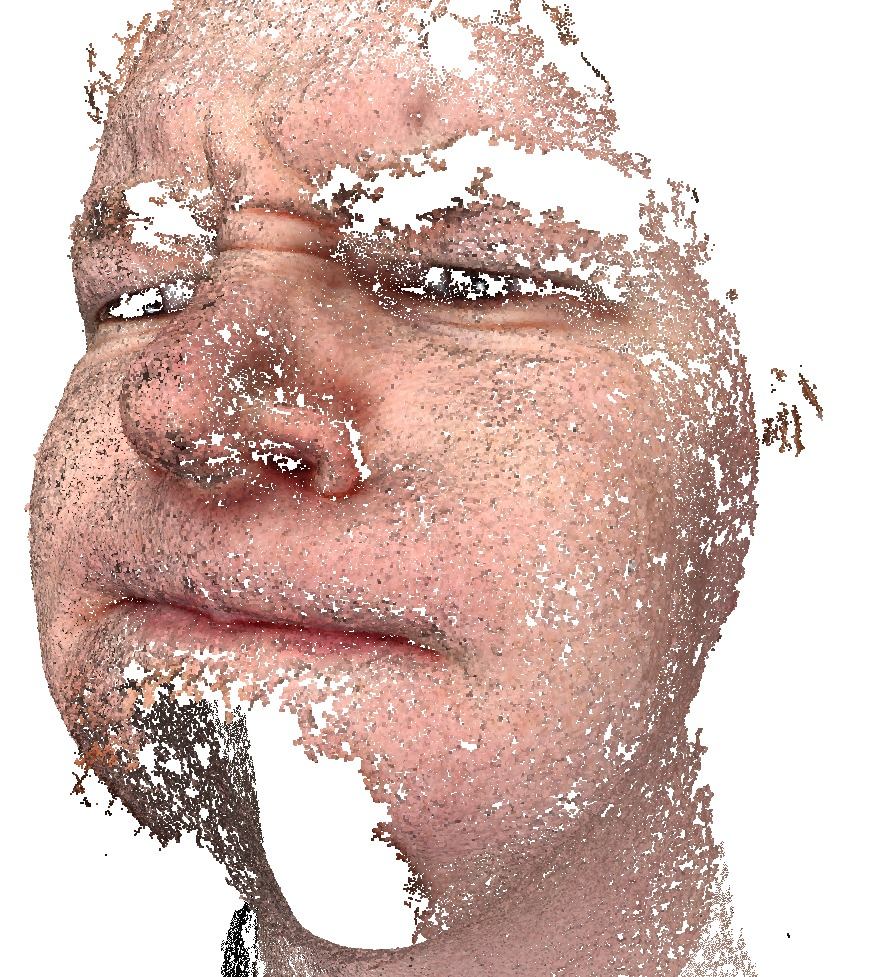
\includegraphics[width=0.5\textwidth]{meshlab-head-pts}%
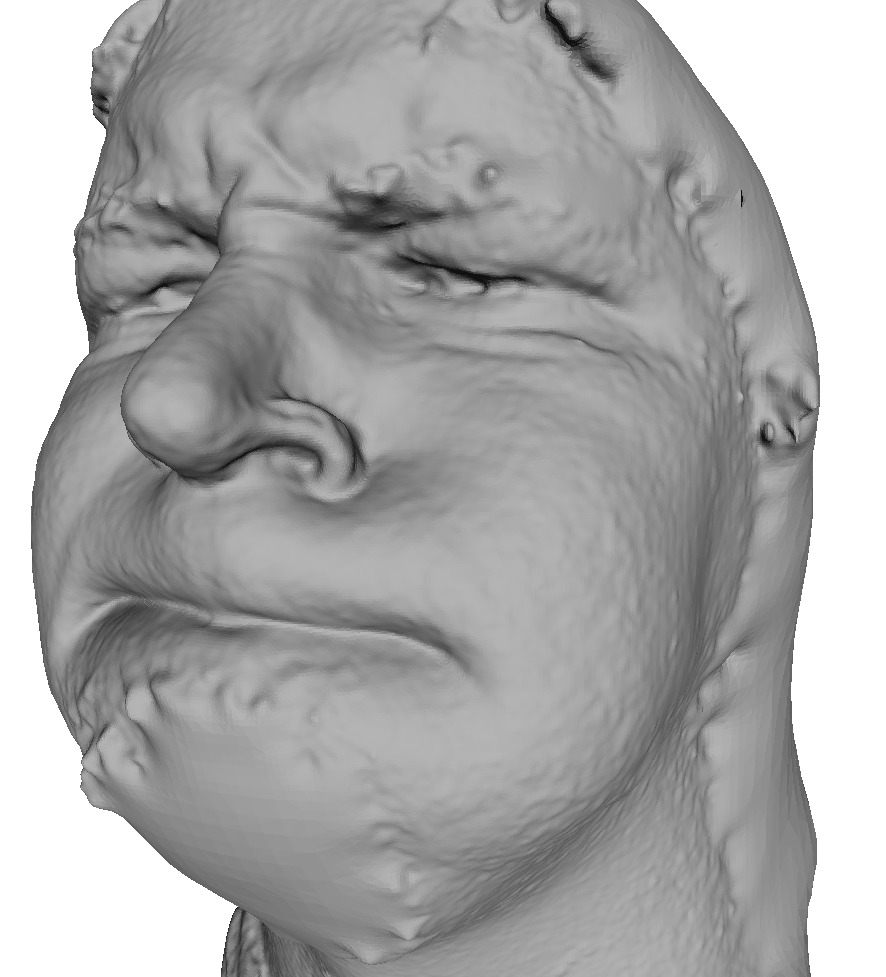
\includegraphics[width=0.5\textwidth]{meshlab-head-solid}\\
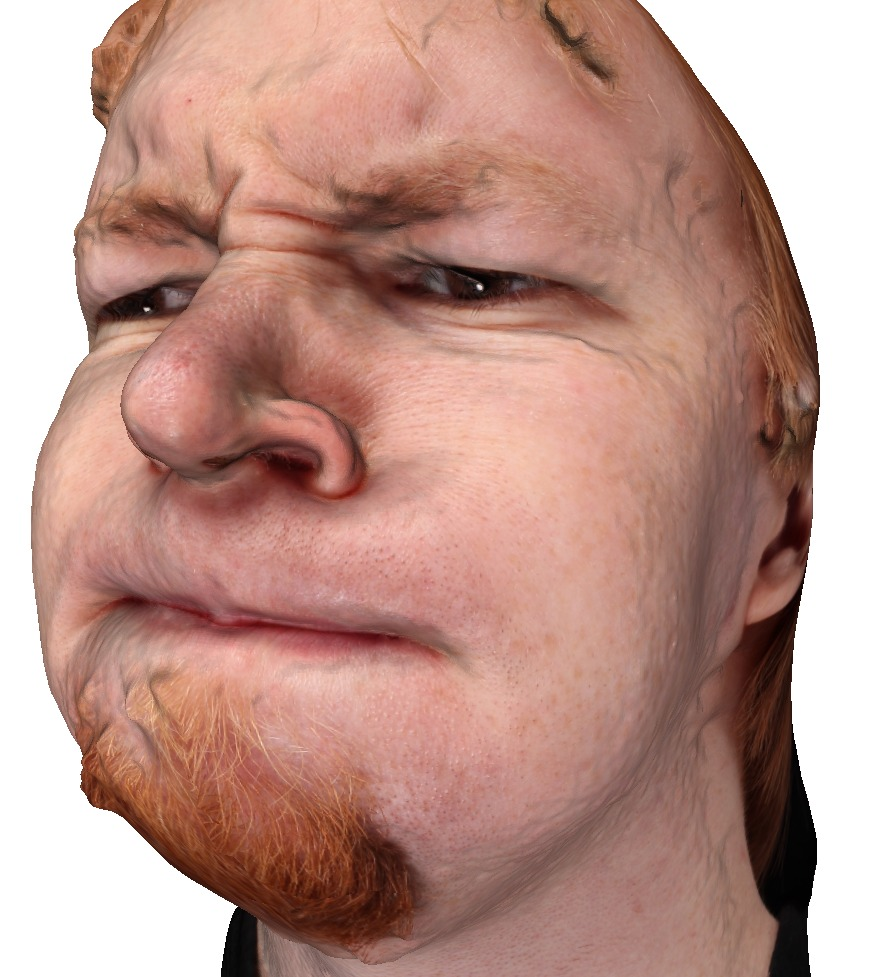
\includegraphics[width=0.5\textwidth]{meshlab-head-tex}%
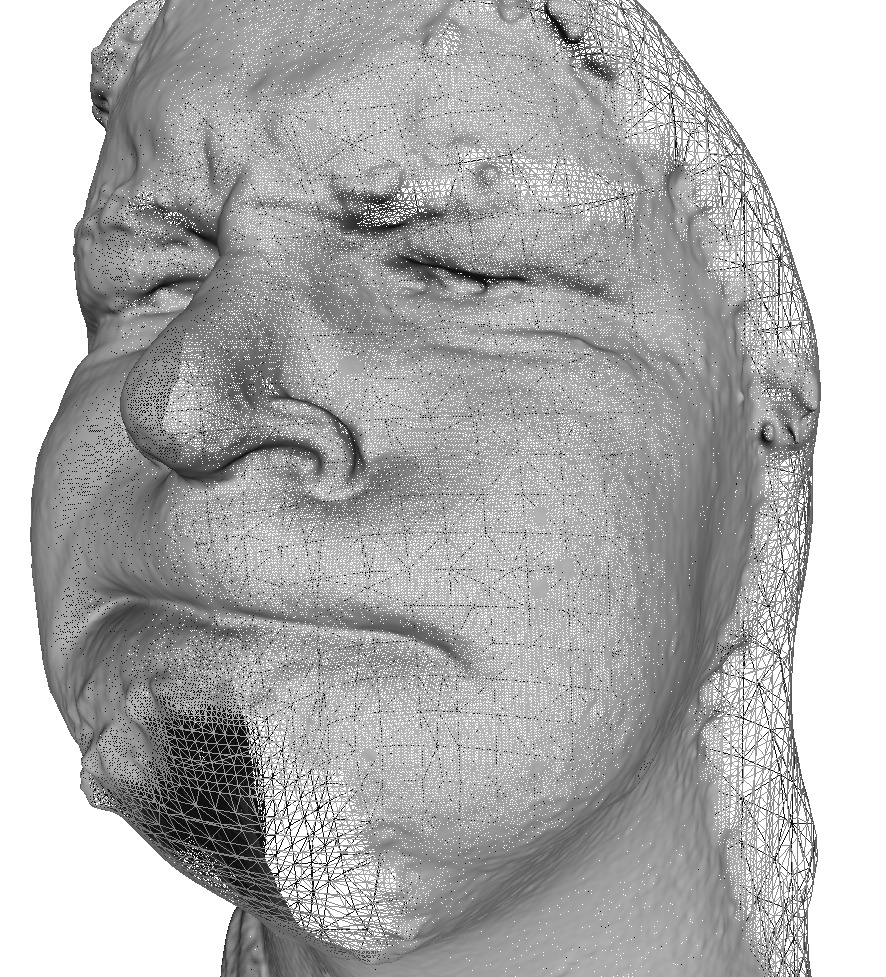
\includegraphics[width=0.5\textwidth]{meshlab-head-wired}
}{fig:sample-sooda-meshlab}{
	A dense point set, solid triangle mesh, textured mesh and a wireframe rendering in Meshlab.
	Point set reconstructed in VisualSFM.
}

\simplefig{h}{%
%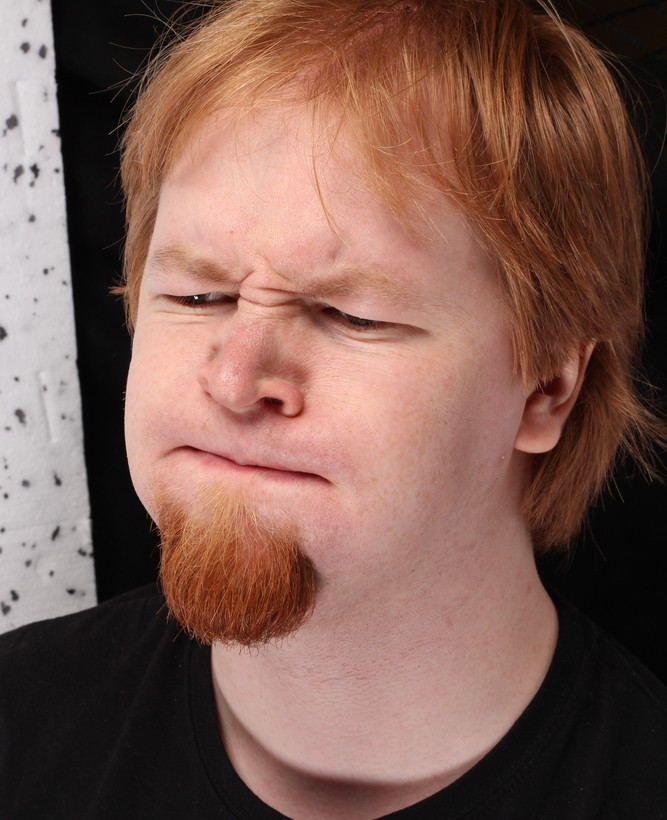
\includegraphics[width=0.38\textwidth]{soodaheadorig}
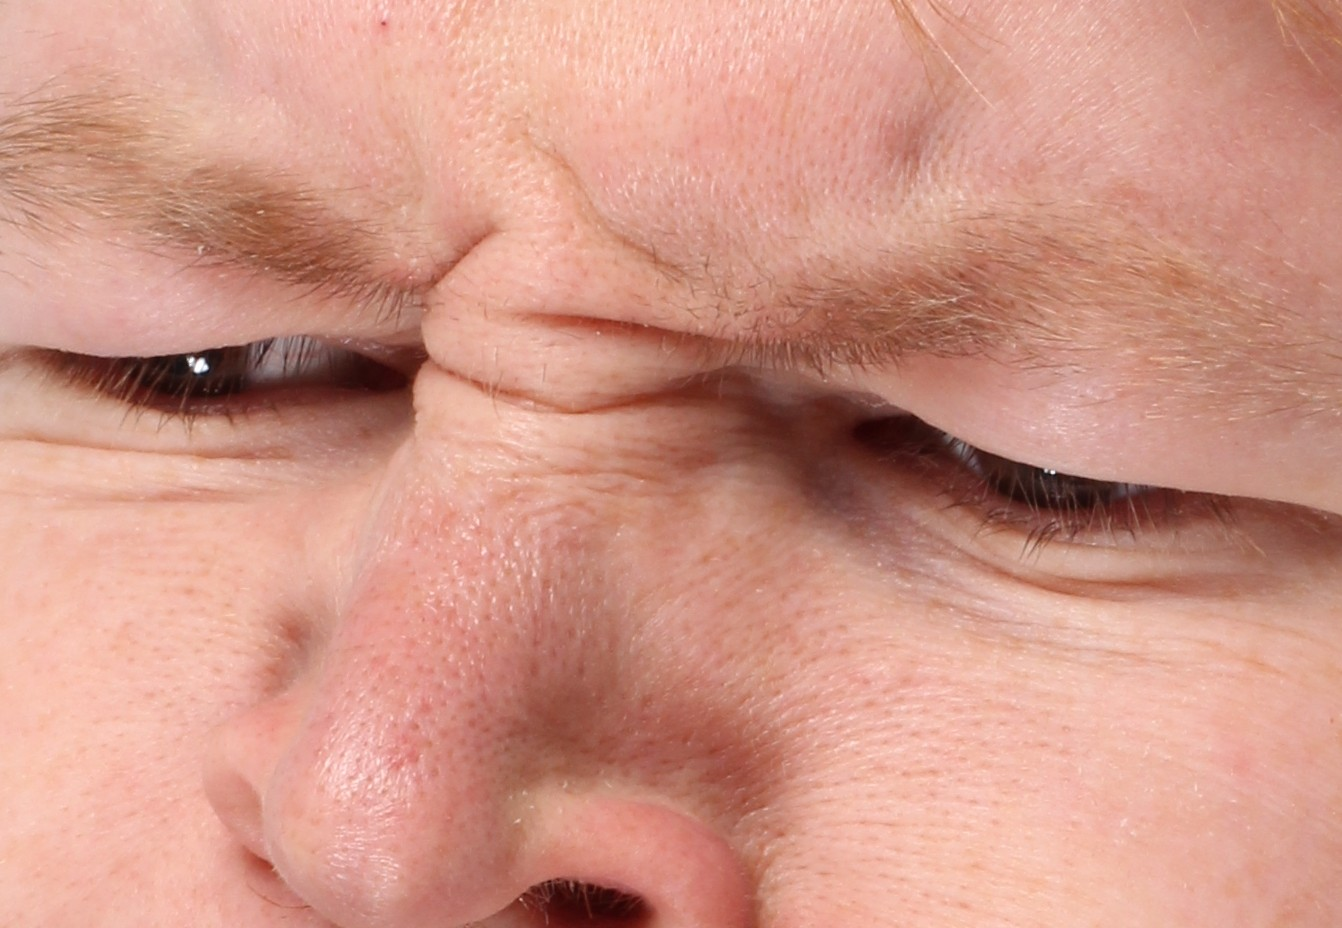
\includegraphics[width=0.9\textwidth]{soodaheadorigclose}
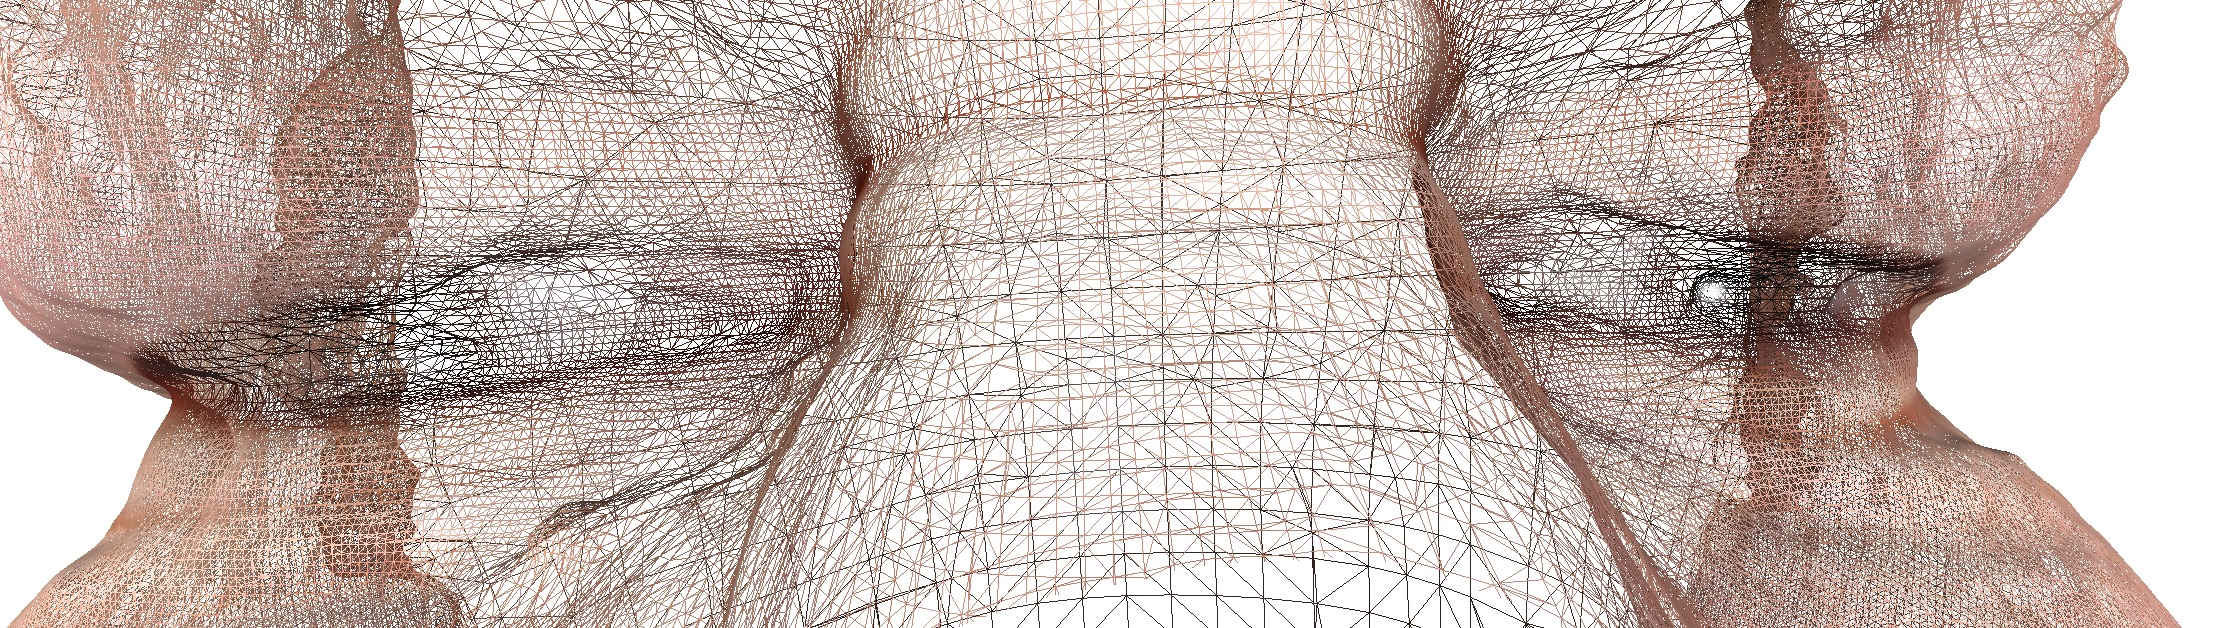
\includegraphics[width=0.9\textwidth]{soodaheadreconsteyeswire}
}{fig:soodaheadclosecompare}{
	Close details from one camera, showing the mesoscopic level of detail, and a corresponding area as a transparent wireframe mesh, showing the amount of vertices.
	Note that the mesh does not yet employ the full geometric properties of the source photograph, i.e.\ the pores and wrinkles, that are beyond the geometric detail of the mesh.
}

\simplefig{h}{%
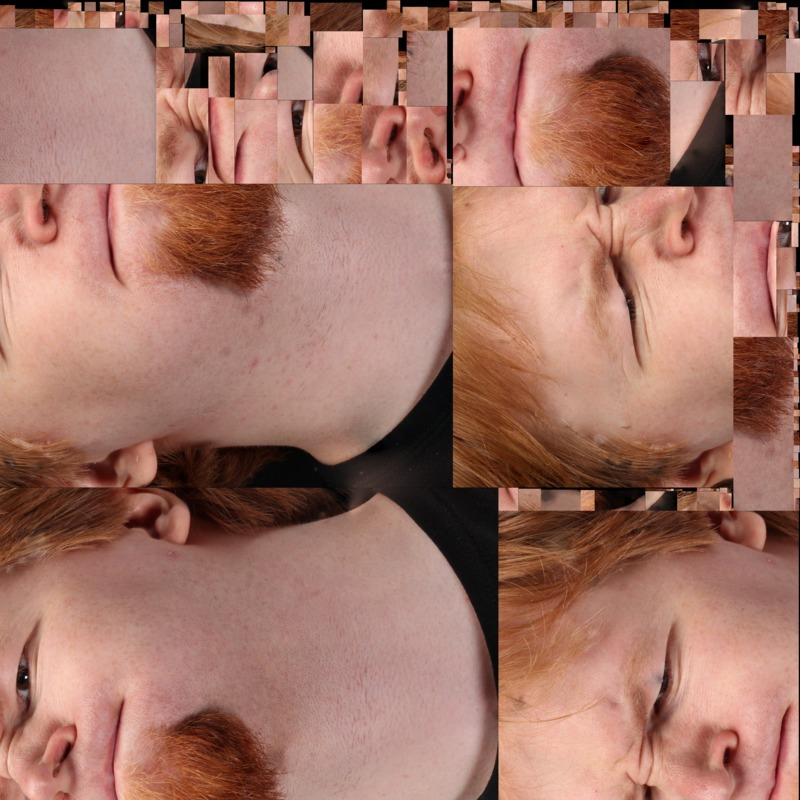
\includegraphics[width=0.7\textwidth]{soodafacetex}%
}{fig:meshlabtex}{
	Meshlab produces a piecewise texture map similar to PhotoScan's generic mode.
}

%\simplegfx{h}{\textwidth}{arto-forehead-uvmap}{
%	Texture map for the model in Figure \ref{fig:sample-arto-forehead}. Note the wrinkle colors in the forehead patches.
%}
%
Other subjects that were also scanned and reconstructed using VisualSFM are summarized in Figure \ref{fig:vsfm-compare}.
Text in a page of a book provides enough dense points that the text is well readable, while the paper itself does not contain any texture and is not reconstructed.
Only problems in human scans are hair that is not well distinguishable (most features are similar) and does not present any definitive surface, and bright spots that result from a combination of bad lighting and sweating.
A horse head mask made of diffuse rubber has problems only in white and black areas that have no texture and either either provide incorrect or no points at all.
Surprisingly, a poorly textured soft plushie provided well reconstructed geometry even in less textured areas, where the fabric provides enough detail to distinguish any correspondences.
A mildly reflective painted statue presented difficulties in some shiny areas, but otherwise, the whole geometry was found to be correct and dense even in visually weakly textured areas.

\simplefig{p}{%
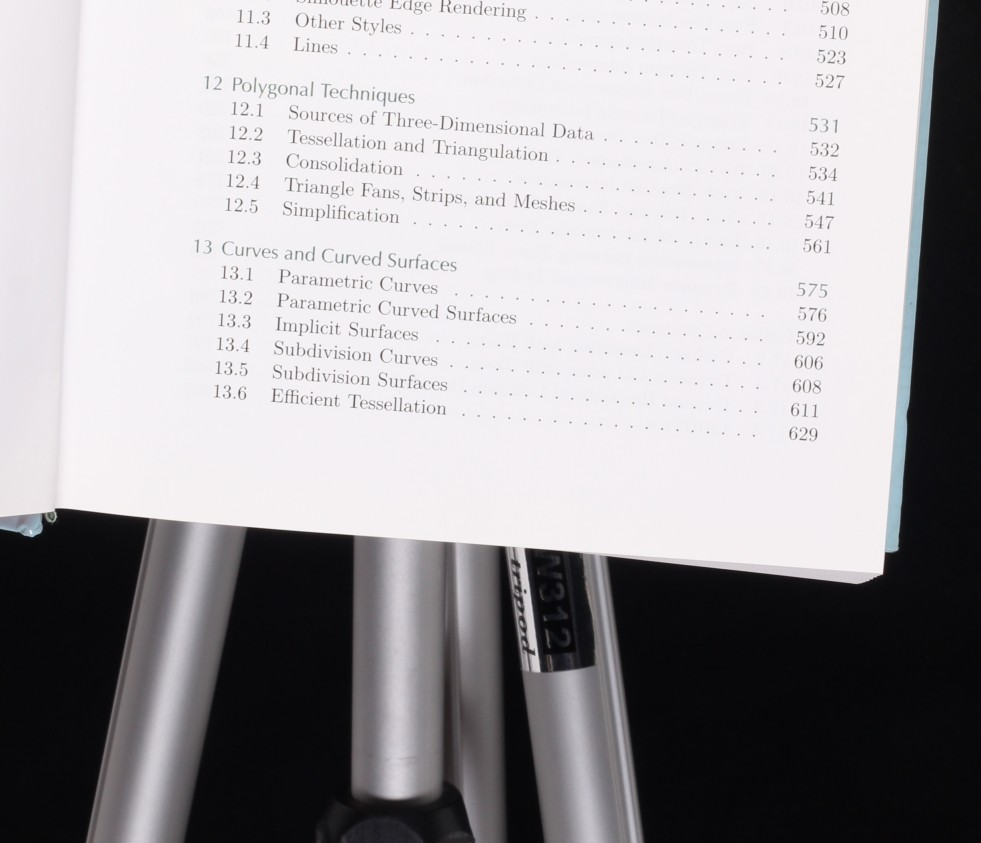
\includegraphics[height=0.22\textheight]{bookorig}
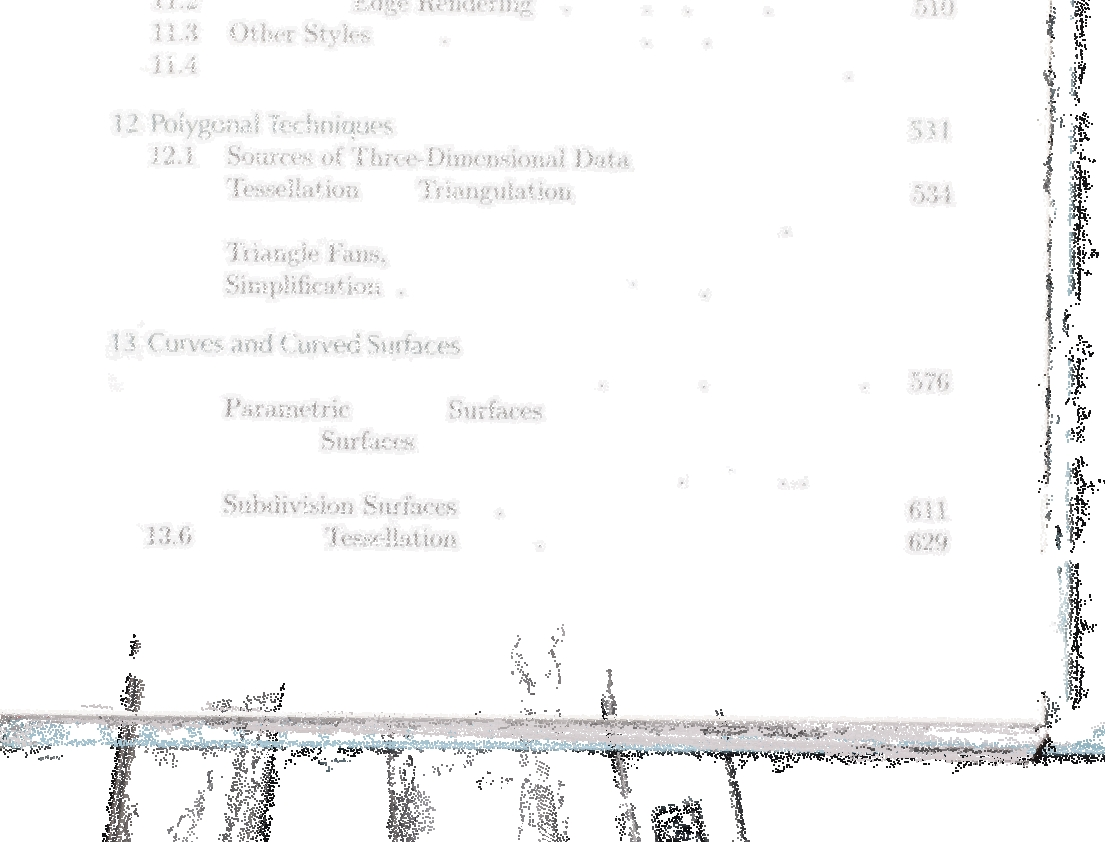
\includegraphics[height=0.22\textheight]{bookreconst}
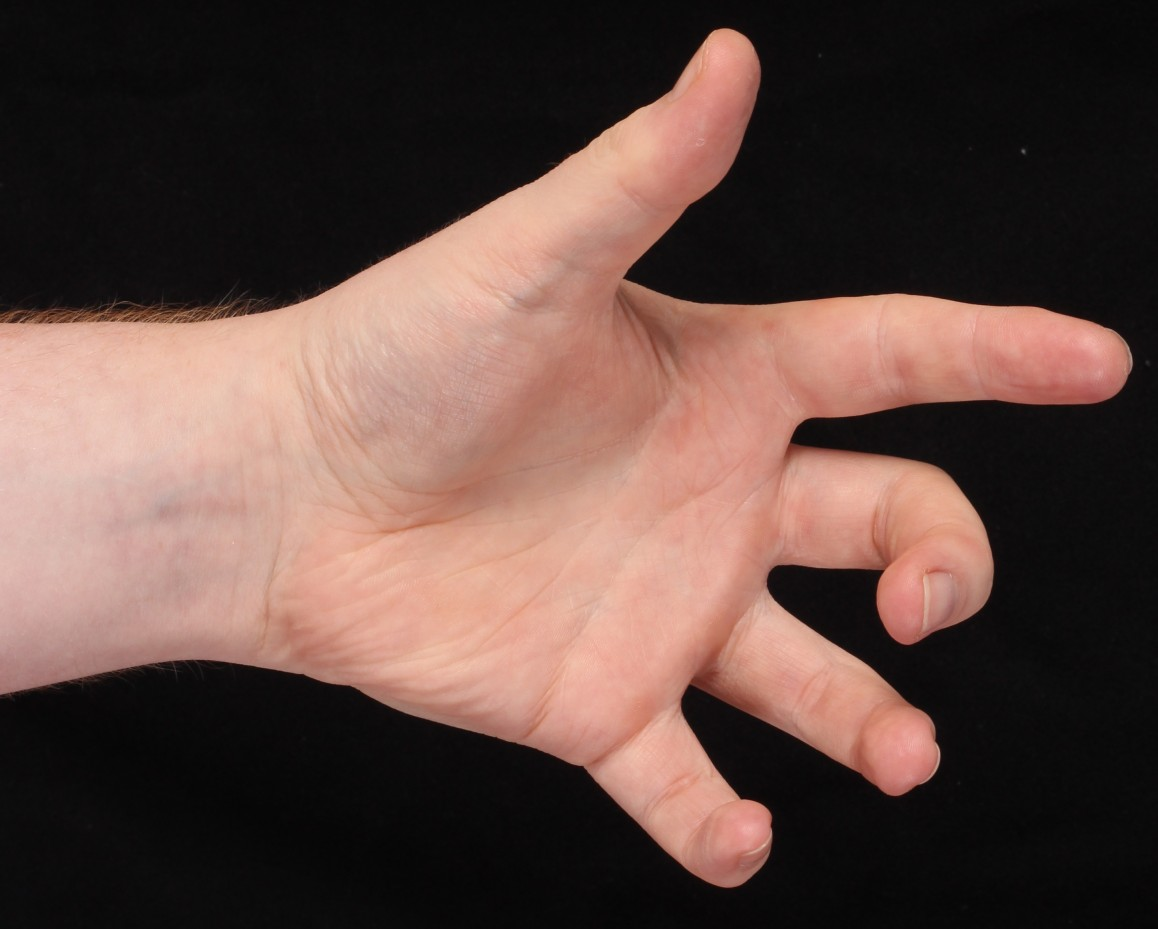
\includegraphics[height=0.22\textheight]{handorig}
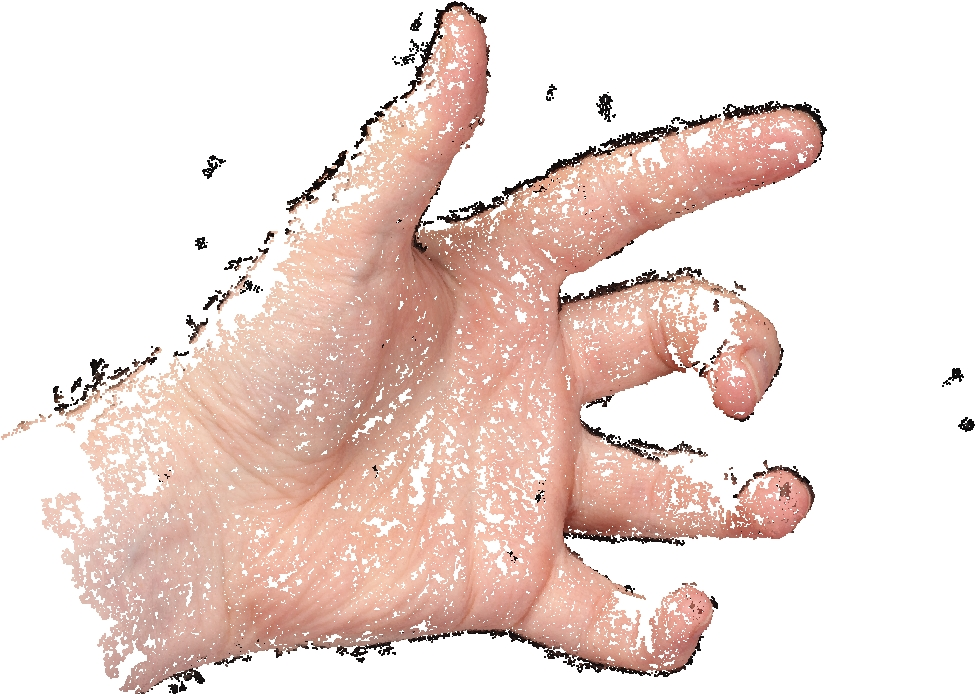
\includegraphics[height=0.22\textheight]{handreconst}
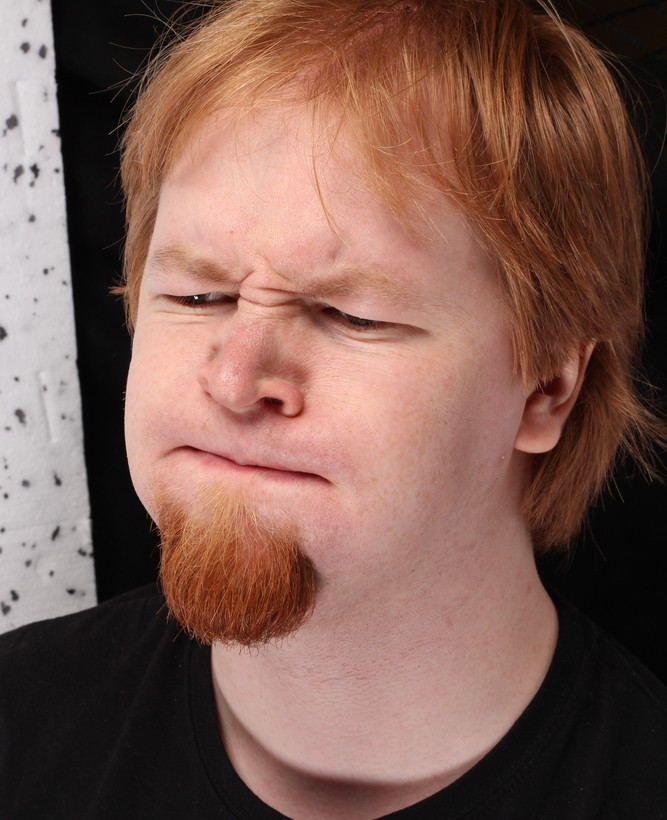
\includegraphics[height=0.22\textheight]{soodaheadorig}
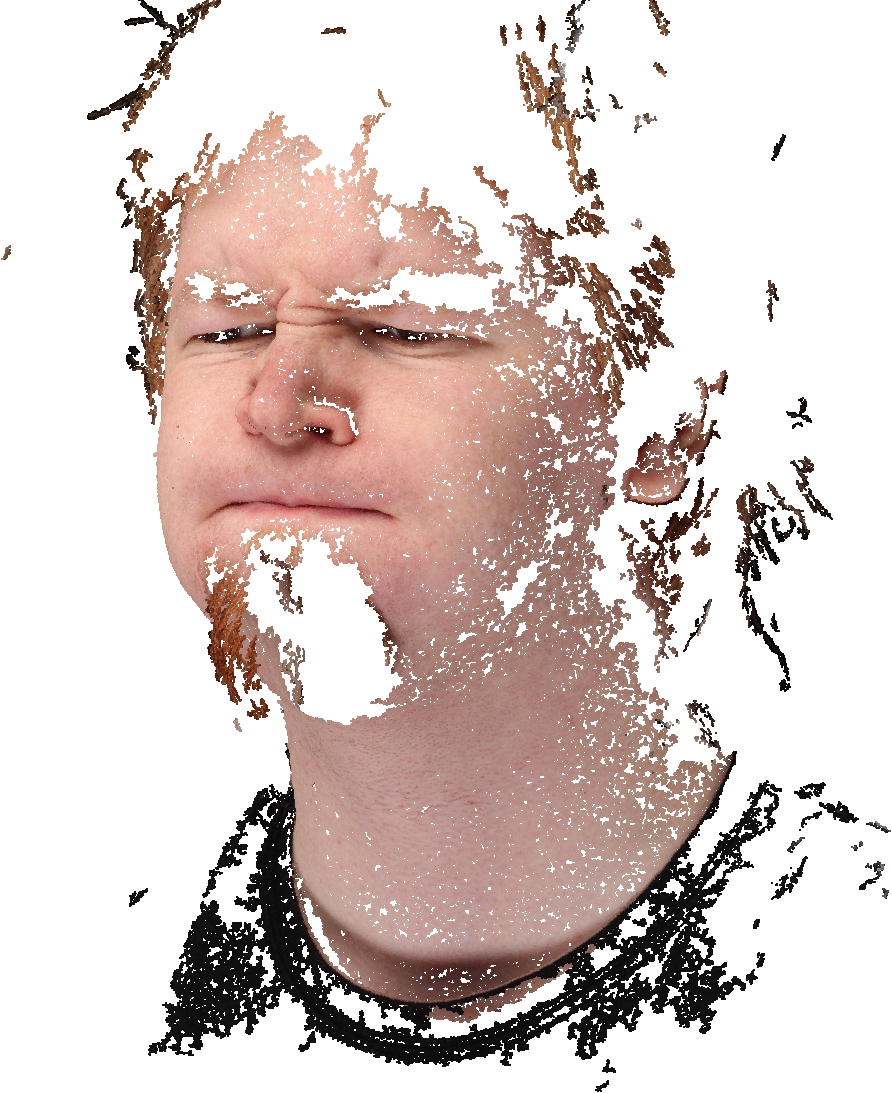
\includegraphics[height=0.22\textheight]{soodaheadreconst}
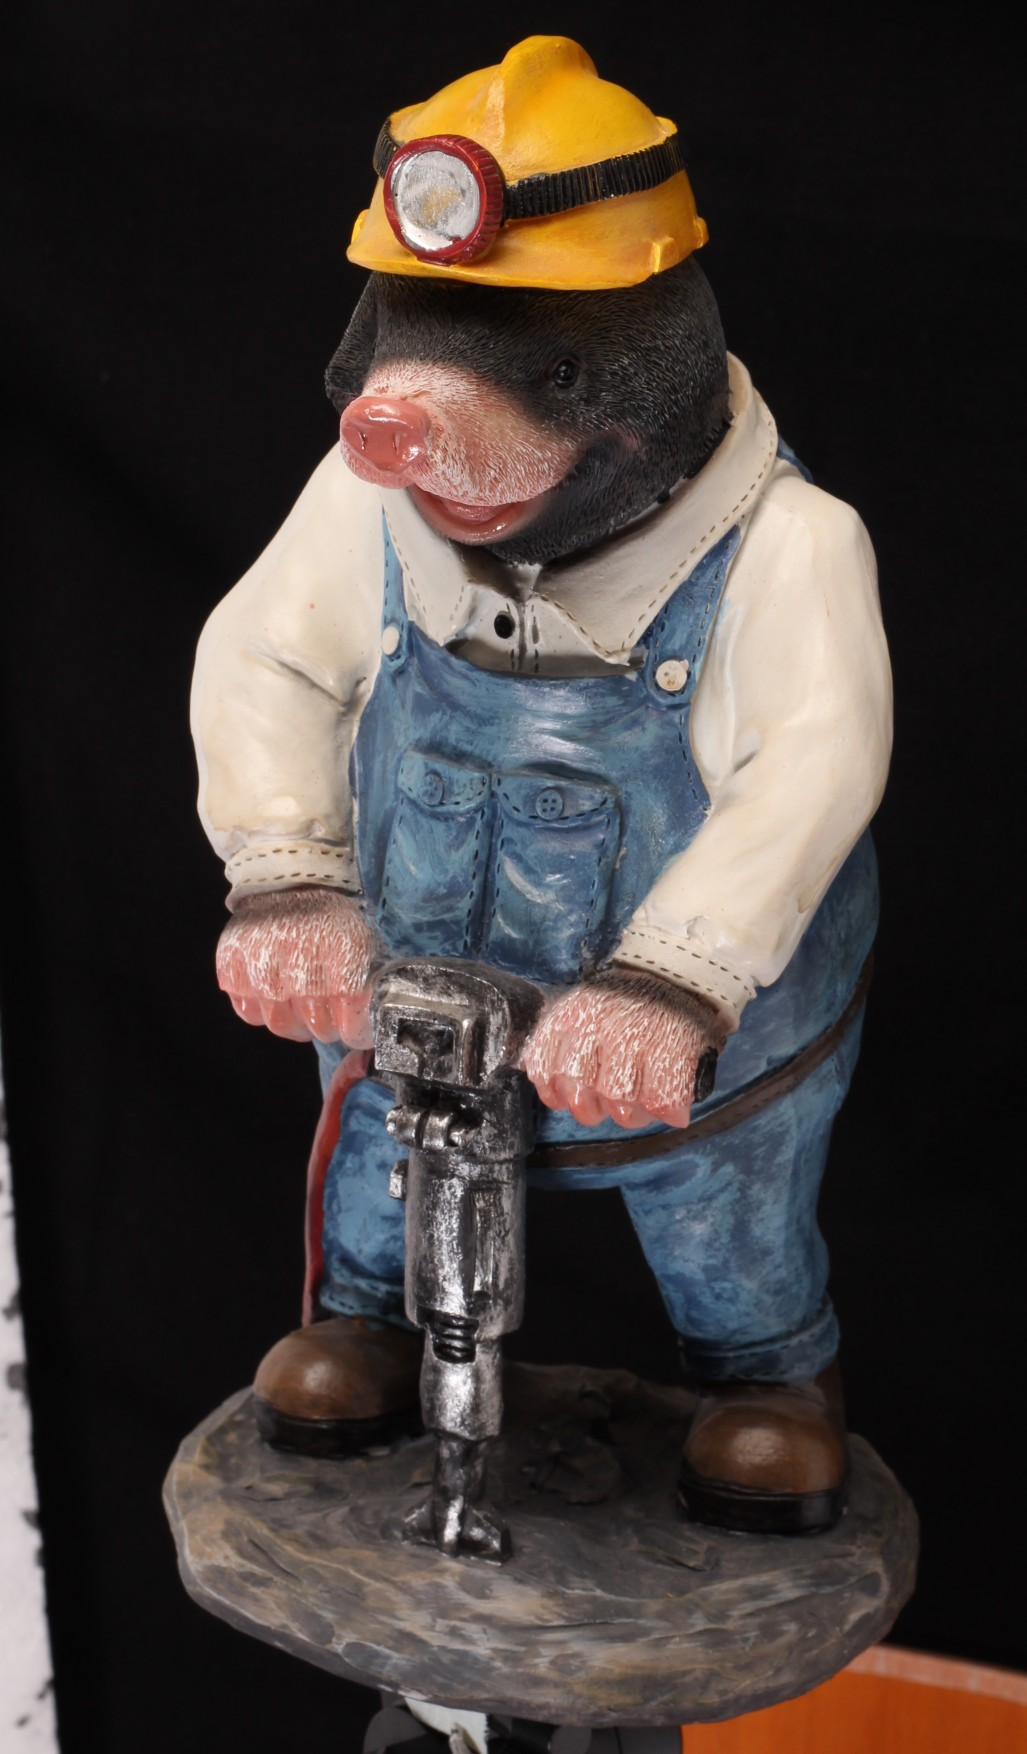
\includegraphics[height=0.22\textheight]{statueorig}
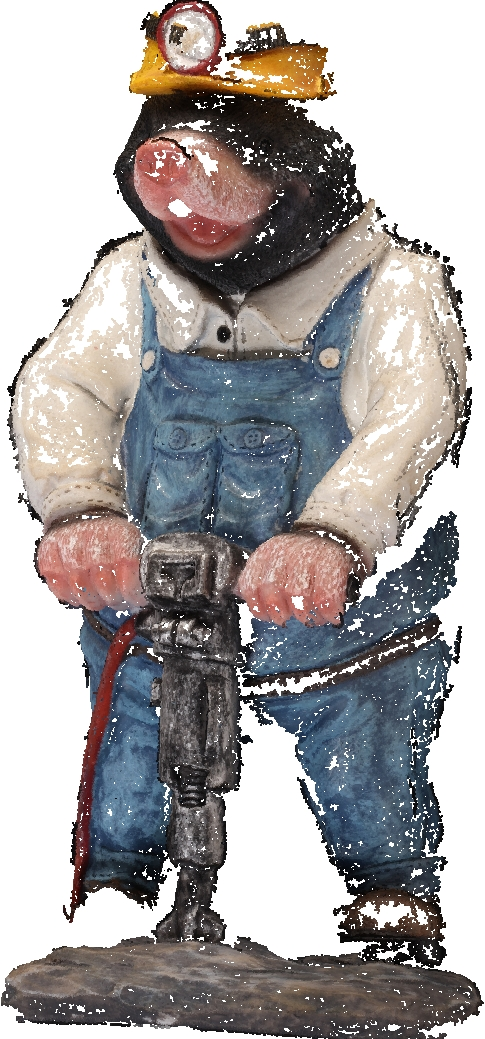
\includegraphics[height=0.22\textheight]{statuereconst}
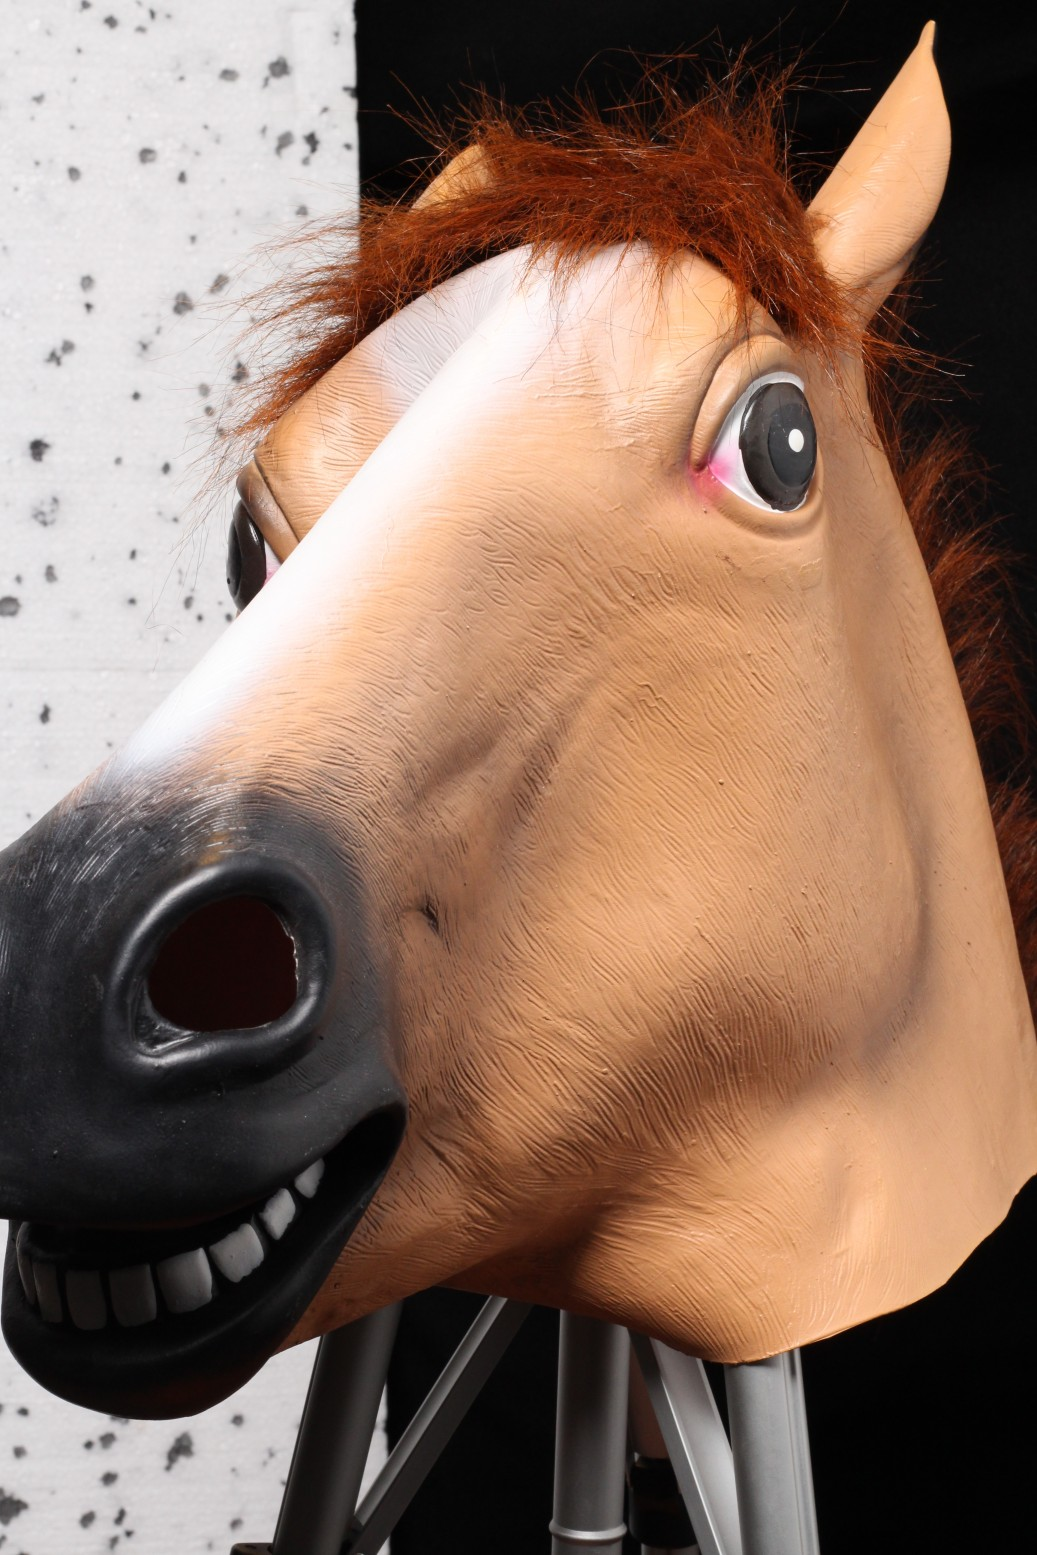
\includegraphics[height=0.22\textheight]{horseorig}
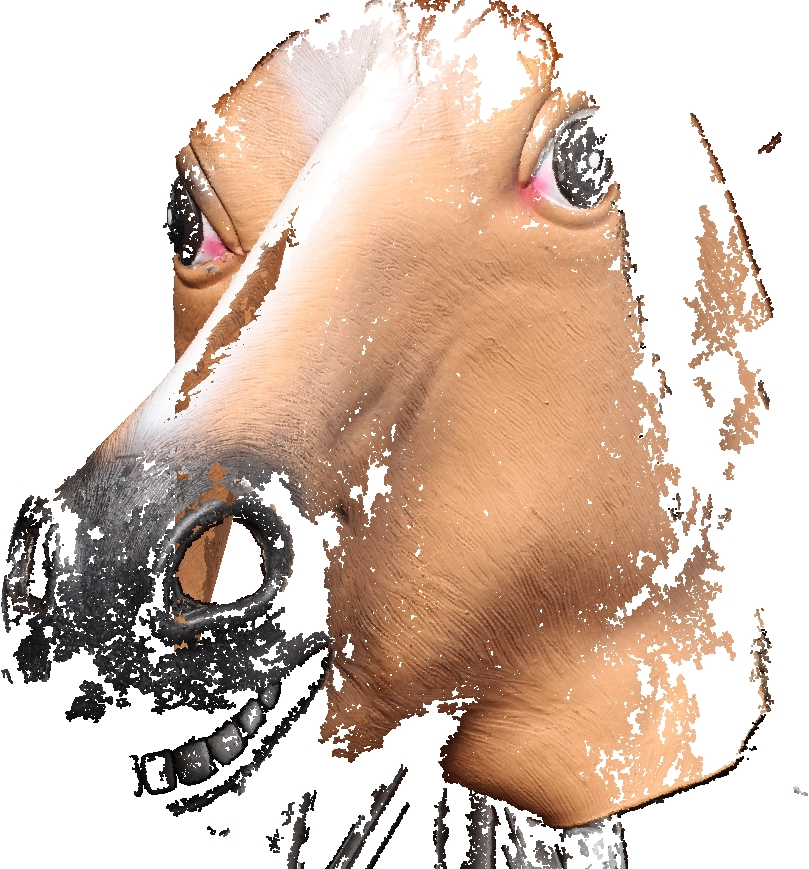
\includegraphics[height=0.22\textheight]{horsereconst}
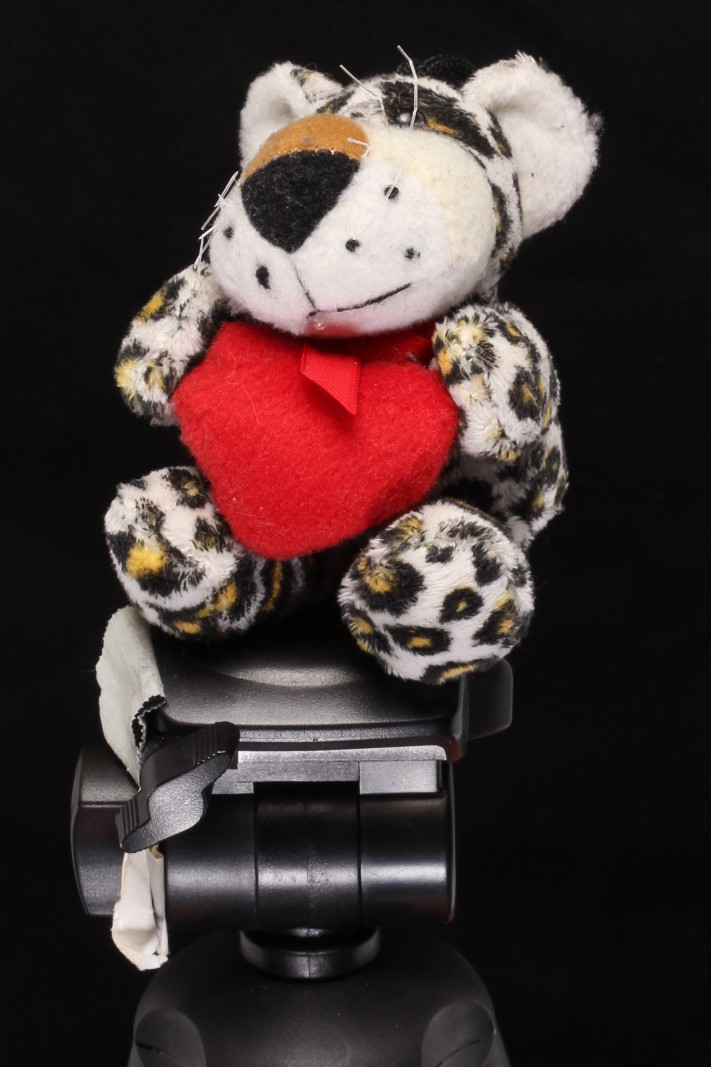
\includegraphics[height=0.22\textheight]{plushieorig}
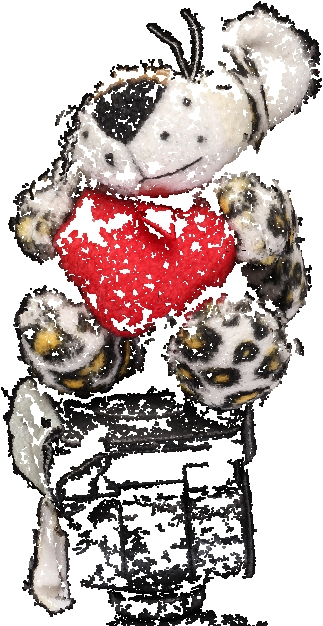
\includegraphics[height=0.22\textheight]{plushiereconst}
}{fig:vsfm-compare}{
	Comparison of original photos and unedited dense point reconstructions done in VisualSFM.
	Subjects listed: book, hand, head, statue, horsemask, plushie.
}

The statue model was scanned four times at approximately 90 degrees of rotation between the shots, and the resulting four point clouds were aligned into one in Meshlab to evaluate a surface reconstruction for a fully closed subject.
Results can be seen in Figure \ref{fig:statue-meshed}.
Some noise exists where it was not cleaned up, and closest details are missing partly because of noise, bright highlight artifacts and selected level of detail in the surface reconstruction.
Slight misalignment in the top can be seen in the point cloud version, and the holes in the bottom are errornously filled in the meshing process.
The mesh was built with Meshlab's Poisson surface reconstruction plugin with 12 as the tree depth and  7 as the solver divide depth.

\simplefig{p}{%
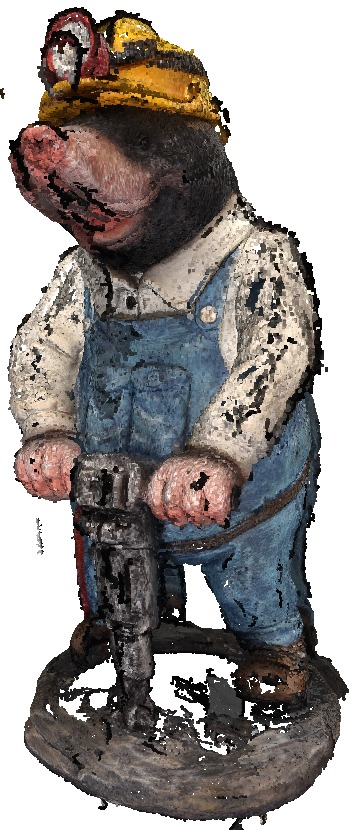
\includegraphics[width=0.5\textwidth]{statue-full-pts}%
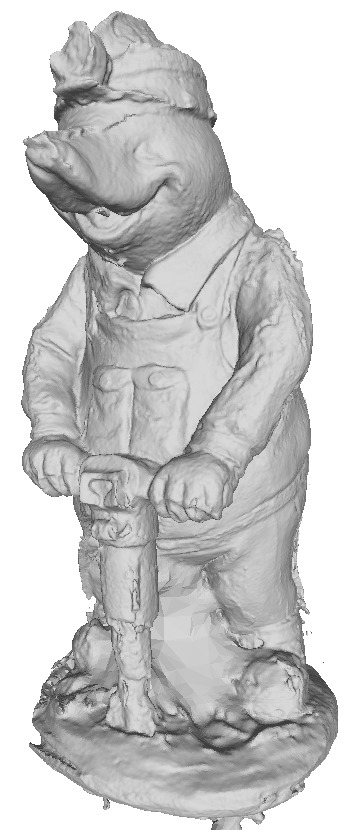
\includegraphics[width=0.5\textwidth]{statue-full-mesh}\\
%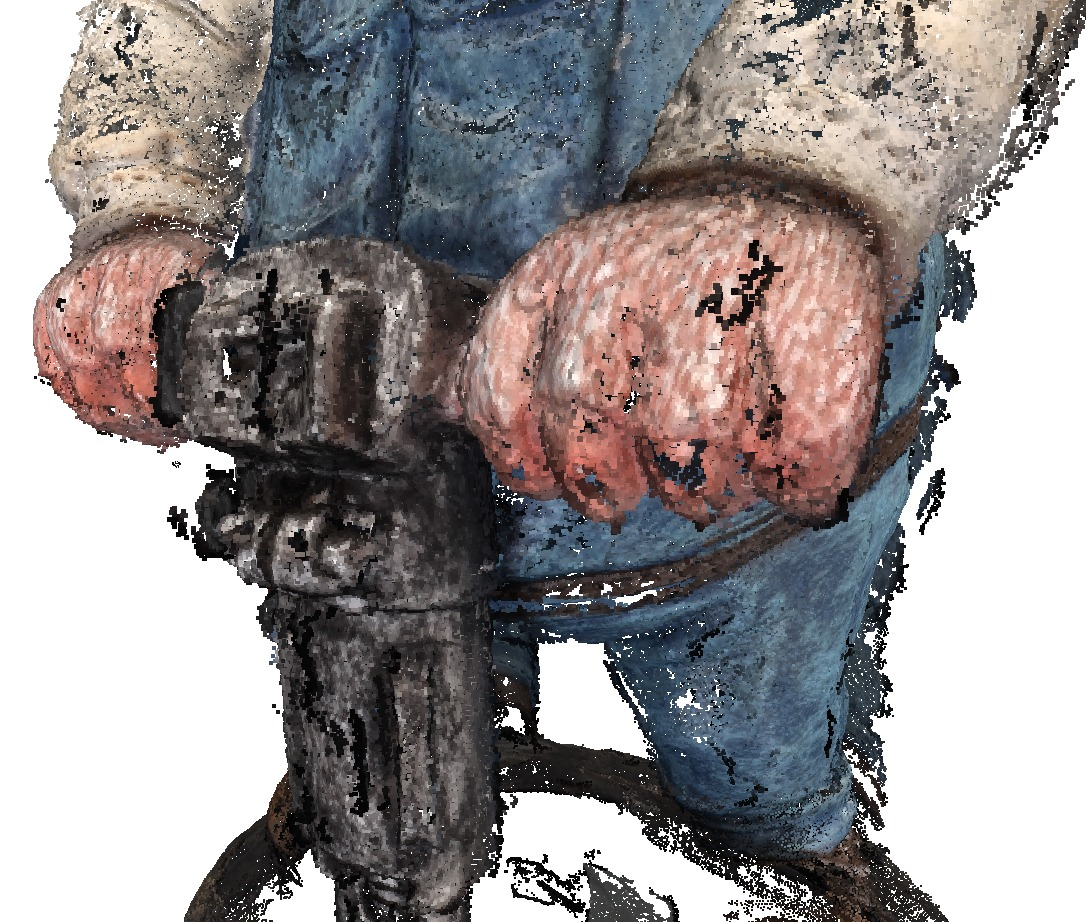
\includegraphics[width=0.5\textwidth]{statue-zoom-pts}%
%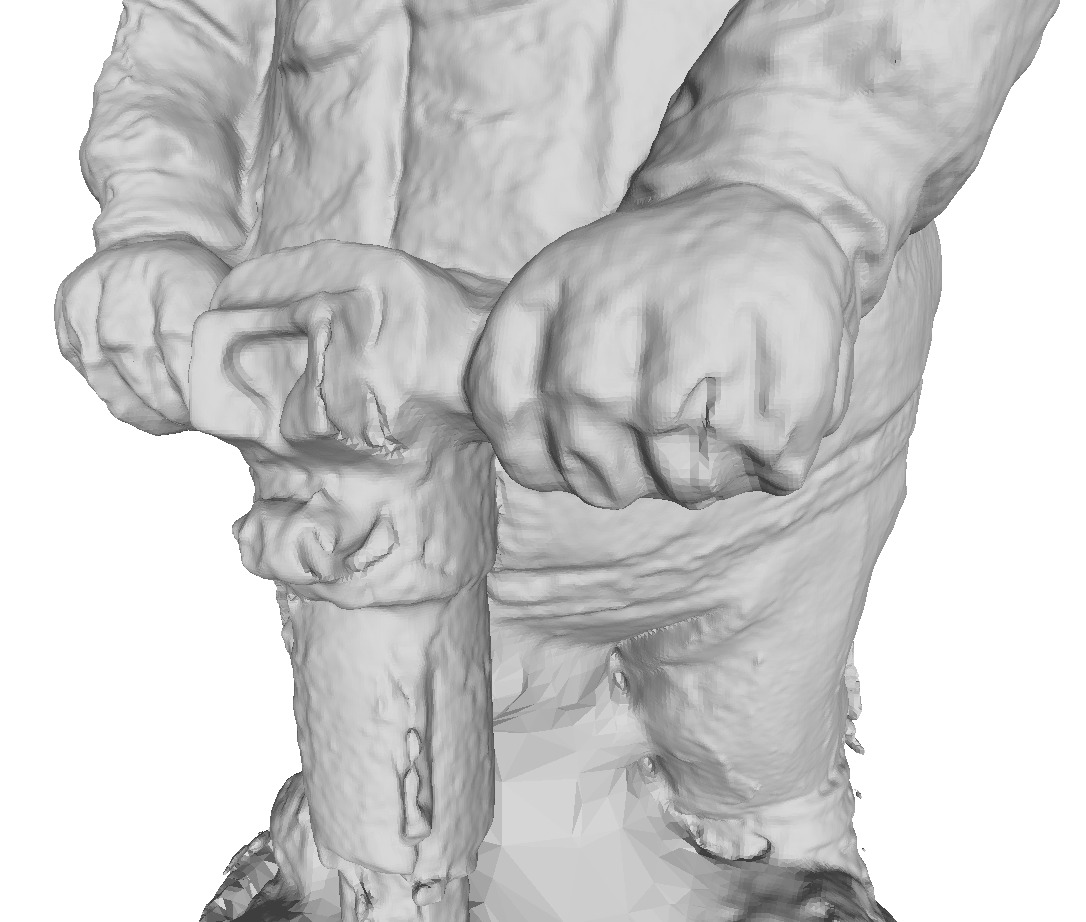
\includegraphics[width=0.5\textwidth]{statue-zoom-mesh}
}{fig:statue-meshed}{
	A full statue as a point set and meshed with Poisson surface reconstruction, combined from four point scans in Meshlab.
	The artifact in the helmet is caused by a slight misalignment between two clouds.
}

%\simplefig{h}{%
%%\includegraphics[width=0.4\textwidth]{meshlab}
%\includegraphics[width=0.4\textwidth]{meshlab}
%\includegraphics[width=0.4\textwidth]{meshlab}
%}{fig:sample-arto-meshlab}{
%	Arto in Meshlab
%}

%A simple lego structure provided to work surprisingly well, even though the lego blocks have a plain color without any texture; the only texture in the structure comes from the corners of different colored blocks.

A simple structure of Lego blocks was scanned with poor results, as was expected; uniform-colored blocks with no texture and no geometry variations present a difficulty to point matching.
The corners between blocks of different color are the only well reconstructed areas.
Figure \ref{fig:legoscompare} depicts the results from three vertical cameras only, as VisualSFM was unable to join the different features of all the cameras.

\simplefig{h}{%
\includegraphics[width=\textwidth]{legosorig}
\includegraphics[width=\textwidth]{legosreconst}
}{fig:legoscompare}{
	A lego block structure demonstrates that textureless surfaces reconstruct poorly, as was expected.
	The old and dirty block in the middle had enough texture to fill better than the others.
}

Typical duration of the reconstruction steps and the used hardware are listed in Table \ref{tab:reconsttime}.
Most of the time is taken by dense reconstruction.
PhotoScan was configured to use CPU only; the dense reconstruction in PMVS is also performed on CPU.
Different approaches remain to be tested; both have a similar working pipeline.

\begin{table}[h]
	% FIXME photoscan here too, it probably performs more work as it takes longer
	\centering
	\begin{tabular}{l l l}
		Step & PhotoScan & VisualSFM+Meshlab \\ \hline
		Feature matching & 75 s & 17 s \\
		SfM / Bundle adjustment & 8 s & 2 s\\
		Undistortion & & 63 s\\
		Dense reconstruction & 40 min & 20 min\\
		Surface reconstruction & 280 s & 90 s\\
		Texturing & 115 s & 15 s\\
	\end{tabular}
	\caption{
		Typical durations of the major reconstruction steps in VisualSFM on an Intel i5-750 CPU and a NVIDIA GeForce GTS 250 GPU.
		The undistortion step is included in the dense reconstruction in PhotoScan.
	}
	\label{tab:reconsttime}
\end{table}

\afterpage{\clearpage}
\subsubsection{Video capture}

Video capture was experimented with three 800 W Inaro Redhead Varibeam spot lights and no significant changes in camera setup, with key parameters listed in Table \ref{tab:samplevideoparams}.
As the cameras may not start recording at the same frame, a small utility was written to rename frames extracted from videos, given a manually set up list of temporal synchronization offsets.
The tool is written in Python and can be found in the source code repository as \emph{sync.py}.

The amount of light needed in video capture can easily be uncomfortable for the performing subject, in contrast to the momentary flash pulse in still photography.
in this experiment, the lights were overly bright and the subject used sunglasses for eye protection; less than three lights resulted in harsh shadows in parts of the face.
the ISO sensitivity level of Canon EOS 700D ranges up to 12800, but the highest levels are usually avoided as they are more sensitive to noise.
A default ``180 degree shutter'' was used, i.e.\ an exposure time of half the time between frames.
A shorter exposure time is suggested with an increased ISO sensitivity to reduce motion blur.

\begin{table}[h]
	\centering
	\begin{tabular}{l l}
		Camera baseline & 30 +/- 5 cm\\
		F number & f/14\\
		Resolution & 1920 x 1080\\
		FPS & 25\\
		Exposure time & 1/50\\
		ISO sensitivity & 800\\
		Subject distance & 90 +/- 10 cm\\
		Lighting & total 2400 W halogen light\\
	\end{tabular}
	\caption{
		Key parameters in the video recording test. % TODO: iso?
	}
	\label{tab:samplevideoparams}
\end{table}

The videos were shot with the larger 50 cm baseline which VisualSFM could not handle; thus, results were analyzed only in PhotoScan.
Incorrect camera poses resulted in some frames, when the subject was moving too quickly; in similar challenging pictures, VisualSFM typically did not reconstruct the parameters at all due to lack of enough matching features.
With less motion, correct camera poses were found and results were comparable to the static reconstruction, with fewer points and polygons reconstructed because of the lower resolution (1920 x 1080).
A typical result is shown in Figure \ref{fig:artoglassescompare}; surface on the textureless and partly reflective sunglasses is incorrect, as was expected.

The camera uses the lossy h.264 video format and typically a bitrate of 5 MB/s.
In comparison, the size taken by a single full-frame JPEG still photo is approximately 9 MB.
The loss in resolution and compression quality results in poor surface details, as is depicted in Figure \ref{fig:artoglassesframe}.

\simplefig{h}{%
\includegraphics[width=0.4\textwidth]{artoglassestex}
\includegraphics[width=0.4\textwidth]{artoglassessolid}
}{fig:artoglassescompare}{
	PhotoScan reconstruction from video frames, textured and solid.
	The solid rendering shows the relatively low vertex count and high amount of spatial noise, which are hidden in this particular textured demonstration view.
}

\simplefig{h}{%
\includegraphics[width=0.3\textwidth]{videoframeface}
\includegraphics[width=0.3\textwidth]{videoframefacepart}
\includegraphics[width=0.3\textwidth]{stillframefacepart}
}{fig:artoglassesframe}{
	Video frame quality comparison for the subject in \ref{fig:artoglassescompare}.
	From left to right: a frame of a single camera, a cropped area from it, and a cropped area from a still photo.
	Note the colored aliasing in the hair and the lack of surface detail in the skin in the cropped frame.
}

